\documentclass[12pt,a4paper]{article}

\usepackage[utf8]{inputenc}
\usepackage[T1]{fontenc}
\usepackage[polish]{babel}
\usepackage{amsmath, amssymb, amsthm}
\usepackage{graphicx}
\usepackage{booktabs}
\usepackage{array}
\usepackage{geometry}
\usepackage{hyperref}
\usepackage{caption}
\usepackage{float}
\usepackage{xcolor}

\geometry{margin=2.5cm}
\graphicspath{{../src/problem_1/figures/}{problem_2/figures/}}

\hypersetup{
    colorlinks=true,
    linkcolor=black,
    urlcolor=blue,
    citecolor=black
}

\title{}
\author{}
\date{}

\begin{document}

\begin{titlepage}
    \centering
    \vspace*{2cm}

    {\Large Politechnika Warszawska}\\[0.3cm]
    {\large Wydział Elektroniki i Technik Informacyjnych}\\[2cm]

    {\large Statystyka w Analizie Danych}\\[0.5cm]
    {\large 01.06.2026}\\[1.5cm]

    \rule{\linewidth}{0.5mm}\\[0.4cm]
    {\huge\bfseries Projekt 2}\\[0.3cm]
    {\Large Testy zgodności rozkładu średniej z rozkładem normalnym\\
    oraz detekcja słabego sygnału w szumie}\\[0.2cm]
    \rule{\linewidth}{0.5mm}\\[2cm]

    \begin{flushright}
        \large
        \textit{Autorzy:}\\[0.4cm]
        Mikołaj Garbowski, nr albumu XXXXXX\\
        Bartłomiej Dmitruk, nr albumu 324911\\
    \end{flushright}

    \vfill
    {\large Warszawa, 2026}
\end{titlepage}

\tableofcontents
\newpage

\section{Problem 1 - CTG, kontynuacja Projektu 1}

\subsection{Metoda rozwiązania problemu}

Zadanie polega na ilościowym ujęciu zbieżności rozkładu średniej arytmetycznej $\bar{X}_n$ niezależnych zmiennych losowych do rozkładu normalnego, wynikającej z Centralnego Twierdzenia Granicznego. O ile w pierwszej części projektu zbieżność ta była pokazywana w sposób obrazowy (histogramy, estymatory jądrowe, dystrybuanty empiryczne, wykresy kwantyl-kwantyl), o tyle w tym problemie należy zbadać ją za pomocą statystycznych testów zgodności i porównać moce trzech klasycznych narzędzi: testu Kołmogorowa-Smirnowa, testu Shapiro-Wilka oraz testu D'Agostino. Wynikiem porównania ma być wskazanie, który test najskuteczniej wykrywa odchylenia rozkładu $\bar{X}_n$ od rozkładu normalnego w analizowanym przypadku. Uzupełnienie analizy stanowi estymacja skośności i kurtozy nadmiarowej $\bar{X}_n$ jako wielkości, na których wprost opiera się statystyka testu D'Agostino.

Wybór rozkładu bazowego padł na rozkład wykładniczy z parametrem $\lambda = 1$, czyli $X \sim \mathrm{Exp}(1)$. Decyzja ta wynika z dwóch przesłanek. Po pierwsze, rozkład wykładniczy jest silnie skośny (skośność równa $2$) i ma kurtozę nadmiarową $6$, dzięki czemu odchylenie $\bar{X}_n$ od rozkładu normalnego dla małych $n$ jest wyraźne, a jednocześnie zanika w znanym tempie. Po drugie, wszystkie istotne momenty są dane wzorami analitycznymi ($\mu = 1$, $\sigma^2 = 1$, $\mathrm{Skew}(\bar{X}_n) = 2/\sqrt{n}$, $\mathrm{ExcessKurt}(\bar{X}_n) = 6/n$), co pozwala bezpośrednio porównać estymaty empiryczne z teorią.

Strukturę eksperymentu opisują dwa różne parametry, których nie należy mylić. Liczba uśrednianych zmiennych $n$ wyznacza próbkę, której średnia ma być testowana - jej rosnące wartości odpowiadają coraz lepszemu dopasowaniu $\bar{X}_n$ do rozkładu normalnego. Liczba średnich $K$, podawana na wejście pojedynczego testu, opisuje, ile niezależnych realizacji $\bar{X}_n$ test otrzymuje naraz; im większe $K$, tym silniejszy test (lepsza zdolność wykrycia odchyleń). Zgodnie z zaleceniem projektowym przyjęto $K = 50$ - umiarkowaną wartość rzędu kilkudziesięciu. Liczba uśrednianych zmiennych przyjmuje wartości $n \in \{2, 3, 5, 7, 10, 15, 20, 30, 50, 70, 100, 200, 500\}$, co pokrywa całą strefę przejścia od małych prób, gdzie odchylenie od normalności jest wyraźne, aż do prób, dla których żaden z testów nie potrafi już rozróżnić $\bar{X}_n$ od $N(\mu, \sigma^2/n)$.

Schemat pojedynczej symulacji wygląda następująco. Dla ustalonego $n$ generowanych jest $K$ niezależnych prób o liczności $n$ z rozkładu $\mathrm{Exp}(1)$ i z każdej obliczana jest średnia arytmetyczna. Otrzymany wektor $K$ średnich stanowi wejście dla trzech testów normalności. Test Kołmogorowa-Smirnowa porównuje dystrybuantę empiryczną standaryzowanych średnich z dystrybuantą $N(0,1)$ przy znanych parametrach $\mu$ oraz $\sigma$, co zapewnia poprawny rozmiar testu i pozwala uniknąć poprawki Lillieforsa. Test Shapiro-Wilka opiera się na statystyce porównującej kombinację liniową statystyk pozycyjnych z wariancją próby i jest powszechnie uznawany za jeden z najmocniejszych testów normalności w niewielkich próbach. Test D'Agostino-Pearsona (statystyka $K^2$) łączy dwa składniki: jeden zależy od skośności, drugi od kurtozy, dzięki czemu test wprost wykrywa najczęstsze formy odejścia od normalności. Całość powtórzono $10\,000$ razy dla każdej wartości $n$, a frakcję odrzuceń hipotezy zerowej przy poziomie istotności $\alpha = 0{,}05$ przyjęto jako estymator mocy.

Aby zweryfikować poprawność implementacji oraz upewnić się, że wszystkie trzy testy utrzymują nominalny poziom istotności, równolegle przeprowadzono symulację kontrolną. W tej wersji $K$ średnich generowano bezpośrednio z rozkładu normalnego $N(0, 1)$ - hipoteza zerowa jest wtedy prawdziwa, a frakcja odrzuceń powinna być bliska $\alpha$. Odchylenia od $0{,}05$ większe niż wynikające z błędu Monte Carlo wskazywałyby na problem z implementacją lub niewłaściwą standaryzacją w teście Kołmogorowa-Smirnowa.

Estymację skośności i kurtozy nadmiarowej $\bar{X}_n$ przeprowadzono osobno, używając $100\,000$ niezależnych realizacji średniej dla każdej wartości $n$. Empiryczne wartości momentów porównano z formułami teoretycznymi $\mathrm{Skew}(\bar{X}_n) = 2/\sqrt{n}$ i $\mathrm{ExcessKurt}(\bar{X}_n) = 6/n$, właściwymi dla bazowego rozkładu $\mathrm{Exp}(1)$. Spadek skośności jak $1/\sqrt{n}$ oraz kurtozy jak $1/n$ odpowiada za stopniowy zanik mocy testu D'Agostino, którego statystyka właśnie z tych dwóch wielkości jest zbudowana.

Symulacje zaimplementowano w języku Python z wykorzystaniem bibliotek \texttt{numpy} oraz \texttt{scipy.stats}; testy wywołują funkcje \texttt{kstest}, \texttt{shapiro} i \texttt{normaltest}. Wszystkie generatory liczb pseudolosowych zainicjalizowano oddzielnymi ziarnami pochodnymi od stałej $\mathrm{SEED} = 42$, dzięki czemu wyniki są w pełni powtarzalne.

\subsection{Wyniki}

\subsubsection{Ilustracja zbieżności $\bar{X}_n$ do rozkładu normalnego}

Punktem wyjścia analizy jest wizualne potwierdzenie, że standaryzowana średnia $Z_n = (\bar{X}_n - \mu)/(\sigma/\sqrt{n})$ rzeczywiście zbiega do $N(0, 1)$ wraz ze wzrostem $n$. Rysunek~\ref{fig:convergence} przedstawia w górnym rzędzie histogramy gęstości $Z_n$ uzyskane ze $100\,000$ niezależnych realizacji dla czterech wybranych wartości $n \in \{2, 10, 50, 200\}$, a w dolnym - odpowiadające im wykresy kwantyl-kwantyl względem rozkładu $N(0, 1)$. Dla $n = 2$ histogram zachowuje wyraźną prawostronną skośność dziedziczoną z rozkładu wykładniczego: wartość modalna leży po lewej stronie zera, prawy ogon jest znacznie wydłużony, a wykres kwantyl-kwantyl odchyla się od prostej w obu krańcach, najmocniej w prawym ogonie. Dla $n = 10$ asymetria histogramu wyraźnie się zmniejsza, a wykres kwantyl-kwantyl niemal pokrywa się z prostą w centralnej części, odchylenia pozostają jednak widoczne w prawym ogonie. Przy $n = 50$ histogram jest praktycznie symetryczny i bardzo dobrze odpowiada krzywej gęstości $N(0, 1)$, a wykres kwantyl-kwantyl tworzy linię praktycznie nieodróżnialną od idealnej diagonali. Dla $n = 200$ dopasowanie jest tak dobre, że żadnym z dwóch sposobów nie sposób gołym okiem stwierdzić odejścia od normalności - i właśnie tu pojawia się potrzeba zastosowania testów statystycznych, które jako jedyne dają obiektywną, ilościową odpowiedź na pytanie, czy odchylenie jest jeszcze wykrywalne.

\begin{figure}[H]
    \centering
    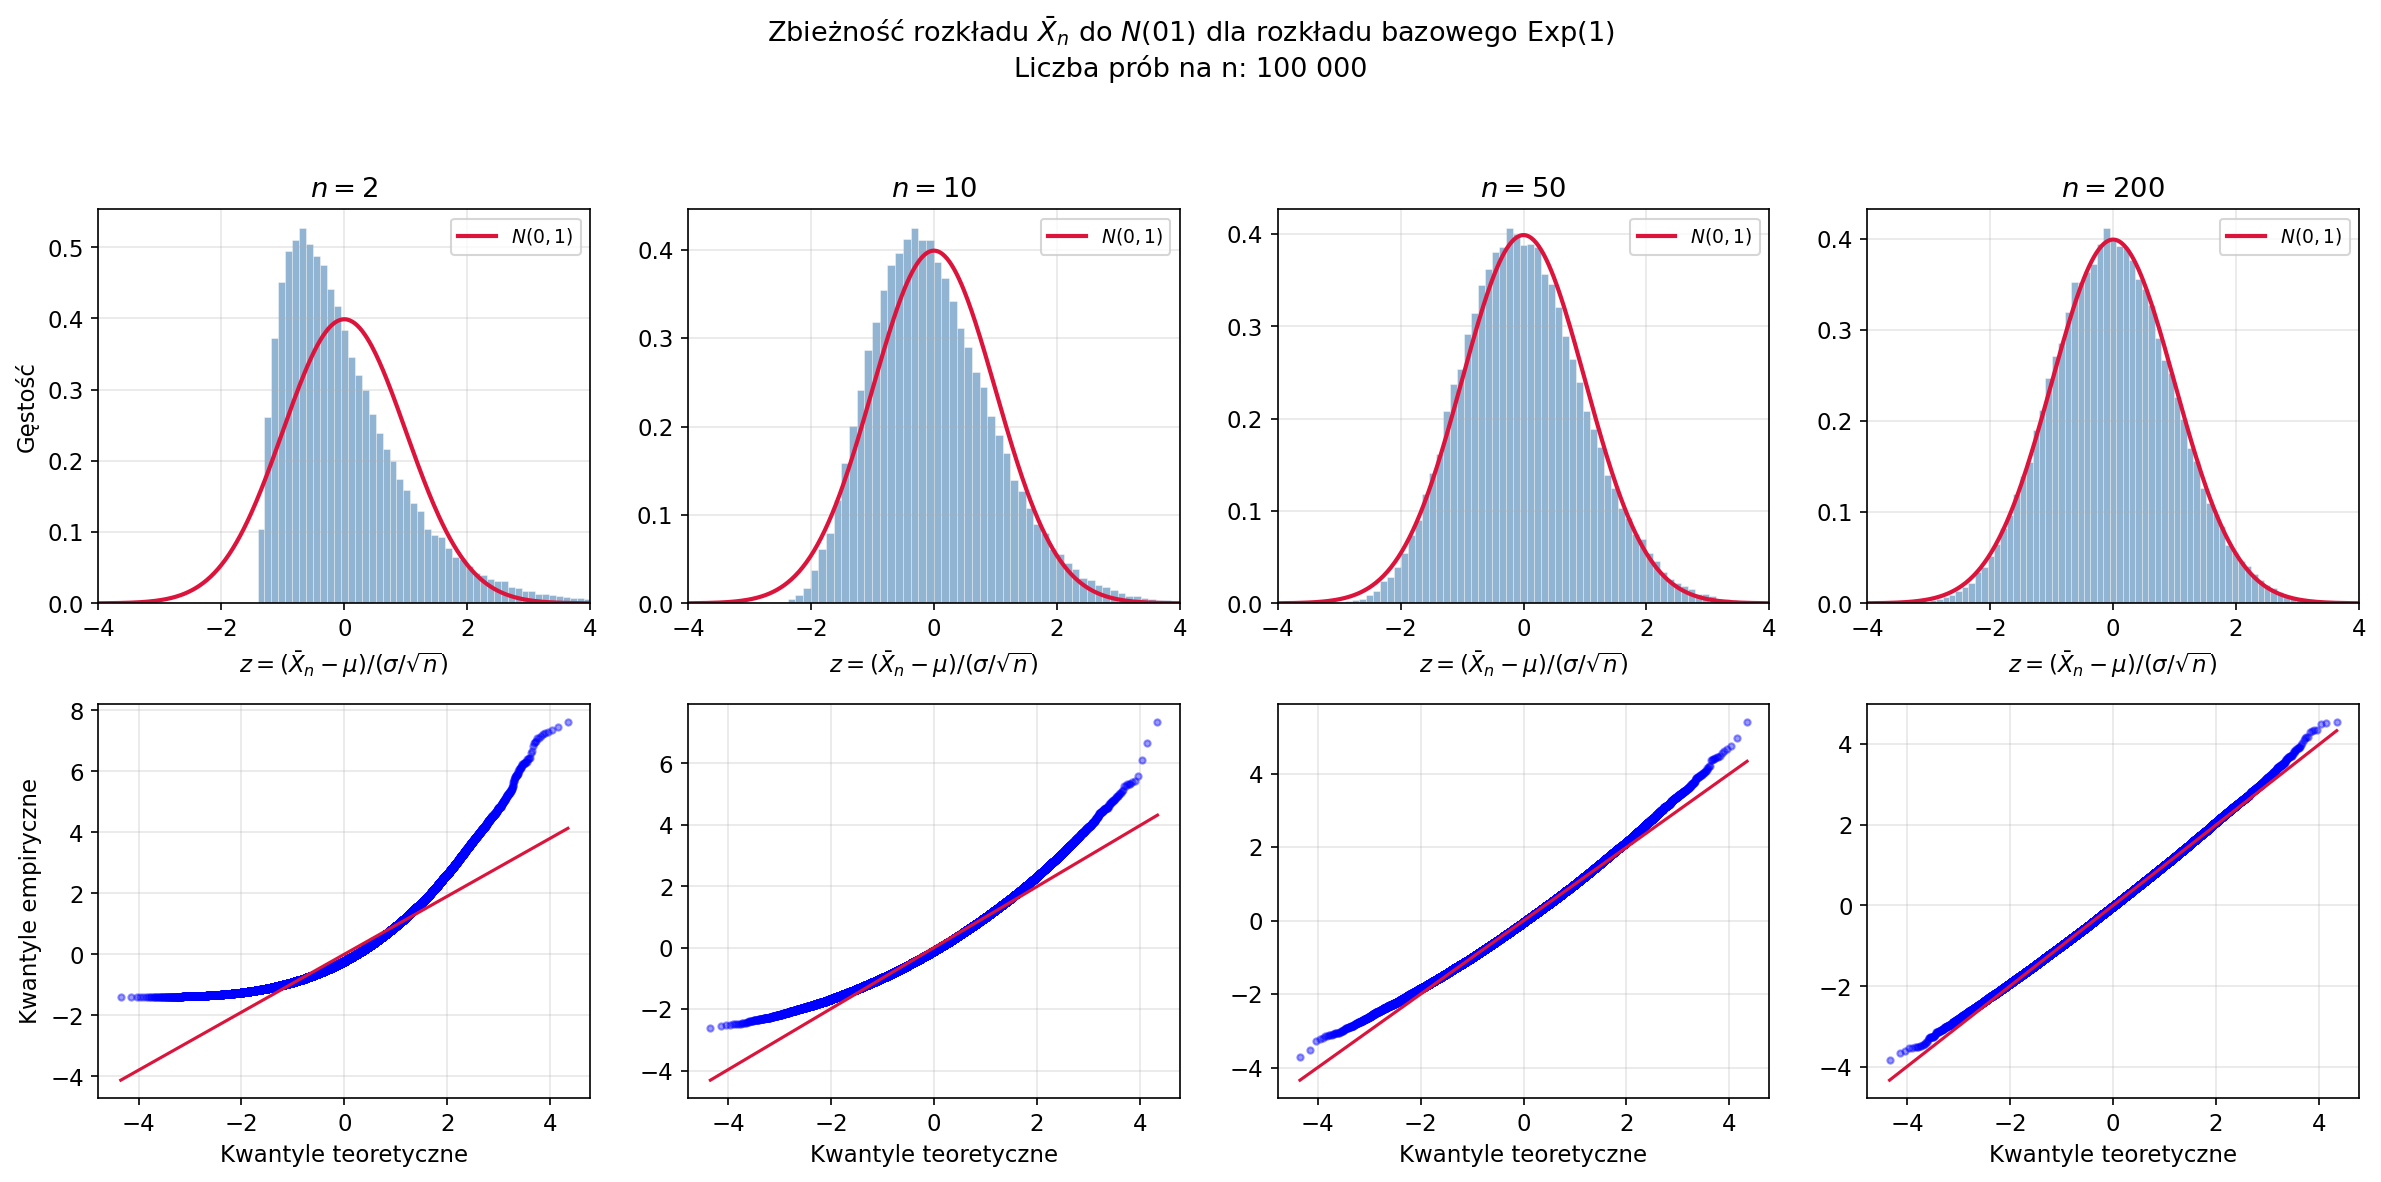
\includegraphics[width=\textwidth]{convergence.png}
    \caption{Zbieżność standaryzowanej średniej $Z_n = (\bar{X}_n - \mu)/(\sigma/\sqrt{n})$ z rozkładu bazowego $\mathrm{Exp}(1)$ do rozkładu $N(0, 1)$. Górny rząd: histogramy gęstości na tle teoretycznej krzywej $N(0, 1)$. Dolny rząd: wykresy kwantyl-kwantyl względem rozkładu $N(0, 1)$.}
    \label{fig:convergence}
\end{figure}

\subsubsection{Moc testów normalności}

Centralny wynik pracy stanowi porównanie mocy trzech testów. Rysunek~\ref{fig:power} pokazuje empiryczną frakcję odrzuceń hipotezy zerowej w funkcji liczby uśrednianych zmiennych $n$, przy stałym $K = 50$ i $\alpha = 0{,}05$. Wszystkie trzy krzywe są monotonicznie malejące - wraz ze wzrostem $n$ rozkład $\bar{X}_n$ coraz lepiej naśladuje rozkład normalny, więc testom jest coraz trudniej wykryć odchylenie od $N(\mu, \sigma^2/n)$.

\begin{figure}[H]
    \centering
    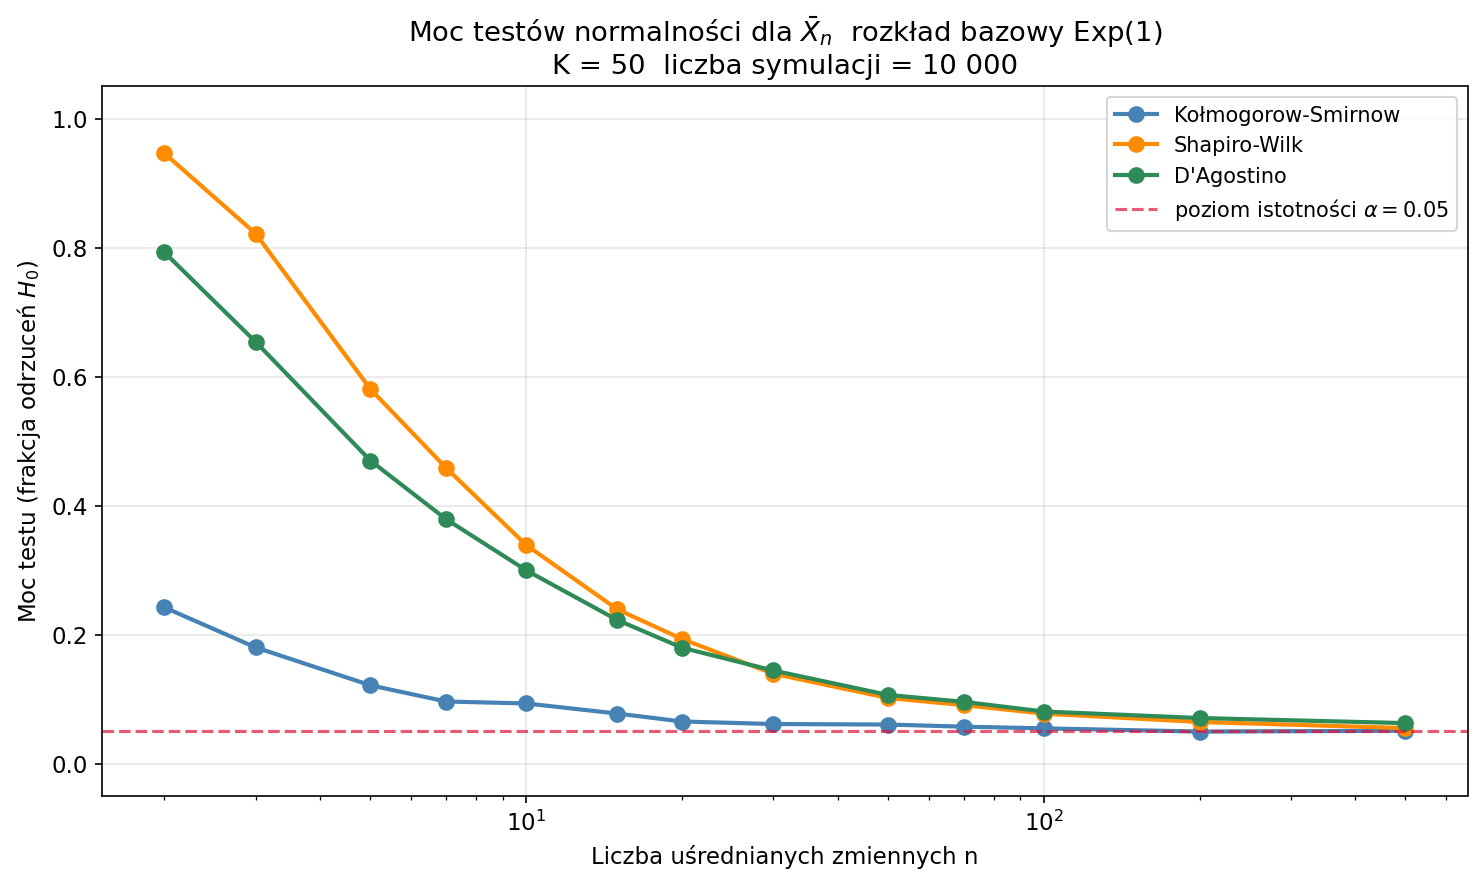
\includegraphics[width=\textwidth]{power_curves.png}
    \caption{Moc testów normalności (frakcja odrzuceń $H_0$) dla średniej $\bar{X}_n$ z rozkładu $\mathrm{Exp}(1)$, $K = 50$, $\alpha = 0{,}05$, $10\,000$ symulacji.}
    \label{fig:power}
\end{figure}

Już z tego rysunku widać wyraźną hierarchię testów. Test Shapiro-Wilka odrzuca hipotezę zerową przy $n = 2$ w niemal 95\% przypadków, podczas gdy test D'Agostino osiąga w tej samej sytuacji moc na poziomie 79\%, a test Kołmogorowa-Smirnowa jedynie nieco ponad 24\%. Hierarchia ta utrzymuje się we wszystkich badanych wartościach $n$, choć przewaga testu Shapiro-Wilka nad D'Agostino jest stała i niewielka, natomiast przewaga obu nad testem Kołmogorowa-Smirnowa jest wielokrotna. Dla $n = 50$, czyli przypadku $K = n$, moce testów Shapiro-Wilka i D'Agostino spadają do około 10\%, a test Kołmogorowa-Smirnowa rejestruje już wartości w okolicach poziomu istotności - dla próby tej długości żaden z testów praktycznie nie odróżnia $\bar{X}_n$ od rozkładu normalnego.

Bliższy widok strefy przejściowej daje rysunek~\ref{fig:power_zoom}, na którym dodano linię referencyjną na poziomie mocy 0{,}5. Pozwala on odczytać, dla jakiej wartości $n$ dany test zachowuje co najmniej połowiczną zdolność wykrycia odchylenia. Test Shapiro-Wilka utrzymuje moc powyżej 0{,}5 do około $n \approx 7$, test D'Agostino nieznacznie krócej - do mniej więcej $n \approx 5$, natomiast moc testu Kołmogorowa-Smirnowa nigdy w badanym zakresie tej granicy nie przekracza i już przy $n = 2$ pozostaje na poziomie ok. 0{,}24.

\begin{figure}[H]
    \centering
    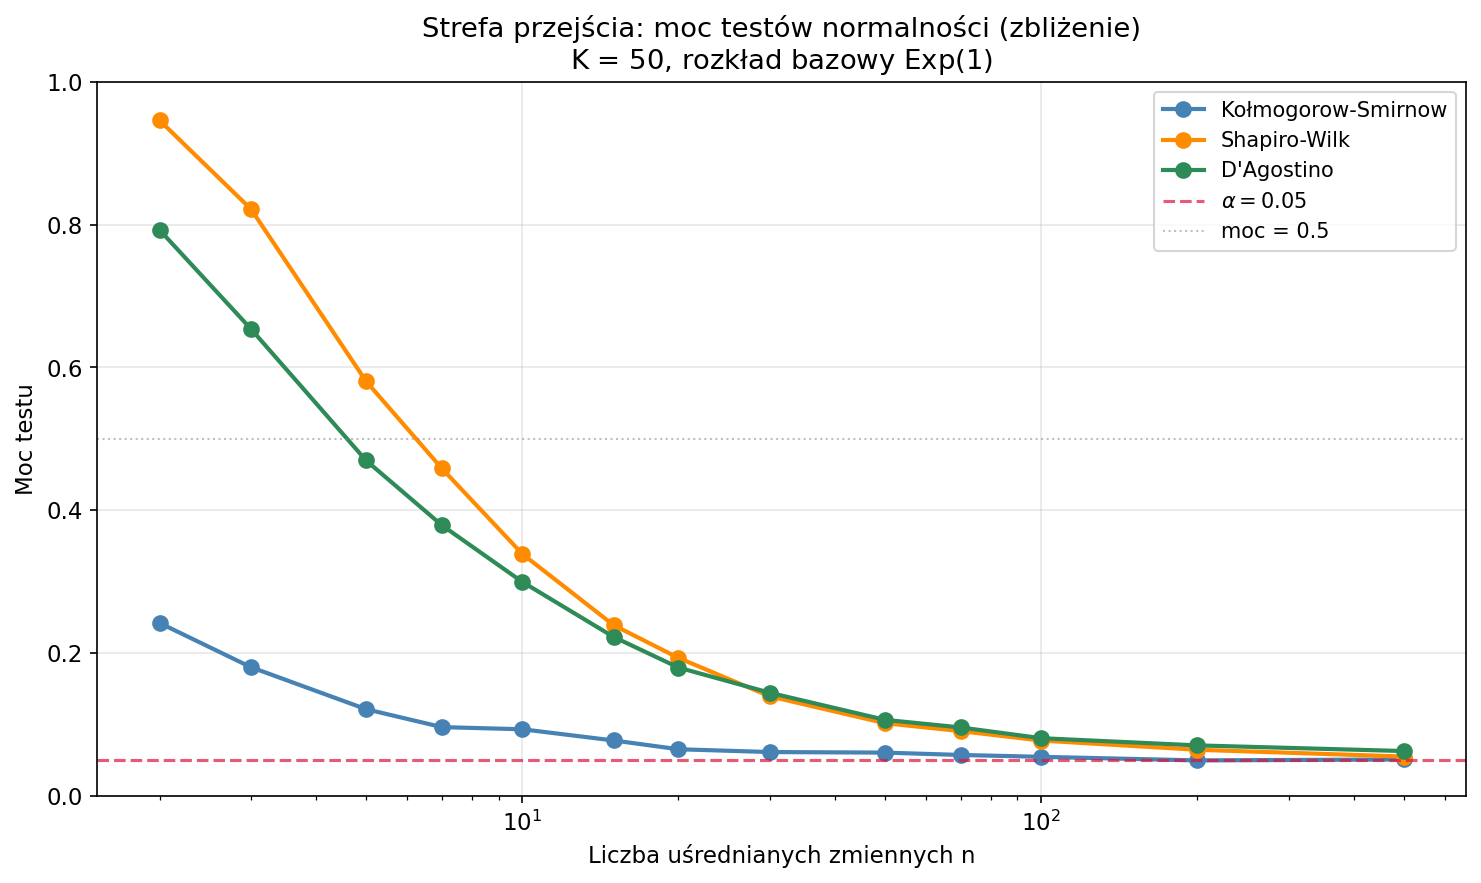
\includegraphics[width=\textwidth]{power_zoom.png}
    \caption{Strefa przejścia mocy testów normalności w pełnym zakresie pionowym z linią referencyjną na poziomie mocy 0{,}5, ułatwiającą porównanie tempa zaniku mocy między testami.}
    \label{fig:power_zoom}
\end{figure}

Pełne wartości liczbowe mocy testów zebrano w tabeli~\ref{tab:power}. W tej samej tabeli umieszczono również wyniki kontroli błędu I rodzaju - frakcję odrzuceń przy danych pochodzących z rozkładu $N(0, 1)$, kiedy hipoteza zerowa jest prawdziwa. Wartości te powinny być bliskie nominalnemu poziomowi istotności $\alpha = 0{,}05$, co rzeczywiście potwierdzają wyniki. Testy Kołmogorowa-Smirnowa i Shapiro-Wilka utrzymują empiryczny rozmiar praktycznie identyczny z nominalnym (różnice mieszczą się w zakresie szumu Monte Carlo), test D'Agostino nieznacznie odrzuca częściej (wartości w przedziale ok. $0{,}055$-$0{,}061$). Pełna zgodność z $\alpha$ stanowi potwierdzenie, że standaryzacja w teście Kołmogorowa-Smirnowa oraz cała procedura symulacyjna są zaimplementowane poprawnie, a różnice w mocach widoczne na rysunku~\ref{fig:power} wynikają faktycznie z odmiennej charakterystyki samych testów, nie z błędu metodologicznego.

\begin{table}[H]
    \centering
    \caption{Moc testów normalności dla danych $\bar{X}_n$ z $\mathrm{Exp}(1)$ oraz empiryczny rozmiar testów dla danych z $N(0, 1)$. $K = 50$, $\alpha = 0{,}05$, $10\,000$ symulacji.}
    \label{tab:power}
    \begin{tabular}{r|rrr|rrr}
\toprule
 & \multicolumn{3}{c|}{Moc (dane z Exp(1))} & \multicolumn{3}{c}{Empiryczny $\alpha$ (dane z $N(0,1)$)} \\
$n$ & KS & SW & D'A & KS & SW & D'A \\
\midrule
2 & 0.242 & 0.946 & 0.792 & 0.048 & 0.053 & 0.059 \\
3 & 0.180 & 0.822 & 0.654 & 0.049 & 0.050 & 0.055 \\
5 & 0.121 & 0.581 & 0.470 & 0.049 & 0.046 & 0.058 \\
7 & 0.096 & 0.459 & 0.379 & 0.050 & 0.054 & 0.058 \\
10 & 0.093 & 0.339 & 0.300 & 0.051 & 0.050 & 0.055 \\
15 & 0.078 & 0.239 & 0.223 & 0.053 & 0.050 & 0.055 \\
20 & 0.065 & 0.193 & 0.180 & 0.052 & 0.049 & 0.057 \\
30 & 0.061 & 0.139 & 0.144 & 0.053 & 0.049 & 0.054 \\
50 & 0.061 & 0.102 & 0.106 & 0.052 & 0.052 & 0.056 \\
70 & 0.057 & 0.091 & 0.096 & 0.049 & 0.051 & 0.059 \\
100 & 0.055 & 0.077 & 0.081 & 0.049 & 0.049 & 0.057 \\
200 & 0.050 & 0.065 & 0.071 & 0.048 & 0.050 & 0.061 \\
500 & 0.051 & 0.055 & 0.063 & 0.052 & 0.051 & 0.057 \\
\bottomrule
\end{tabular}

\end{table}

Rysunek~\ref{fig:type1} przedstawia te same liczby w postaci wykresu. Empiryczne rozmiary testów stabilnie oscylują wokół poziomu $0{,}05$ niezależnie od $n$, co świadczy o tym, że żaden z testów nie traci poprawności dla próbek o liczności $K = 50$.

\begin{figure}[H]
    \centering
    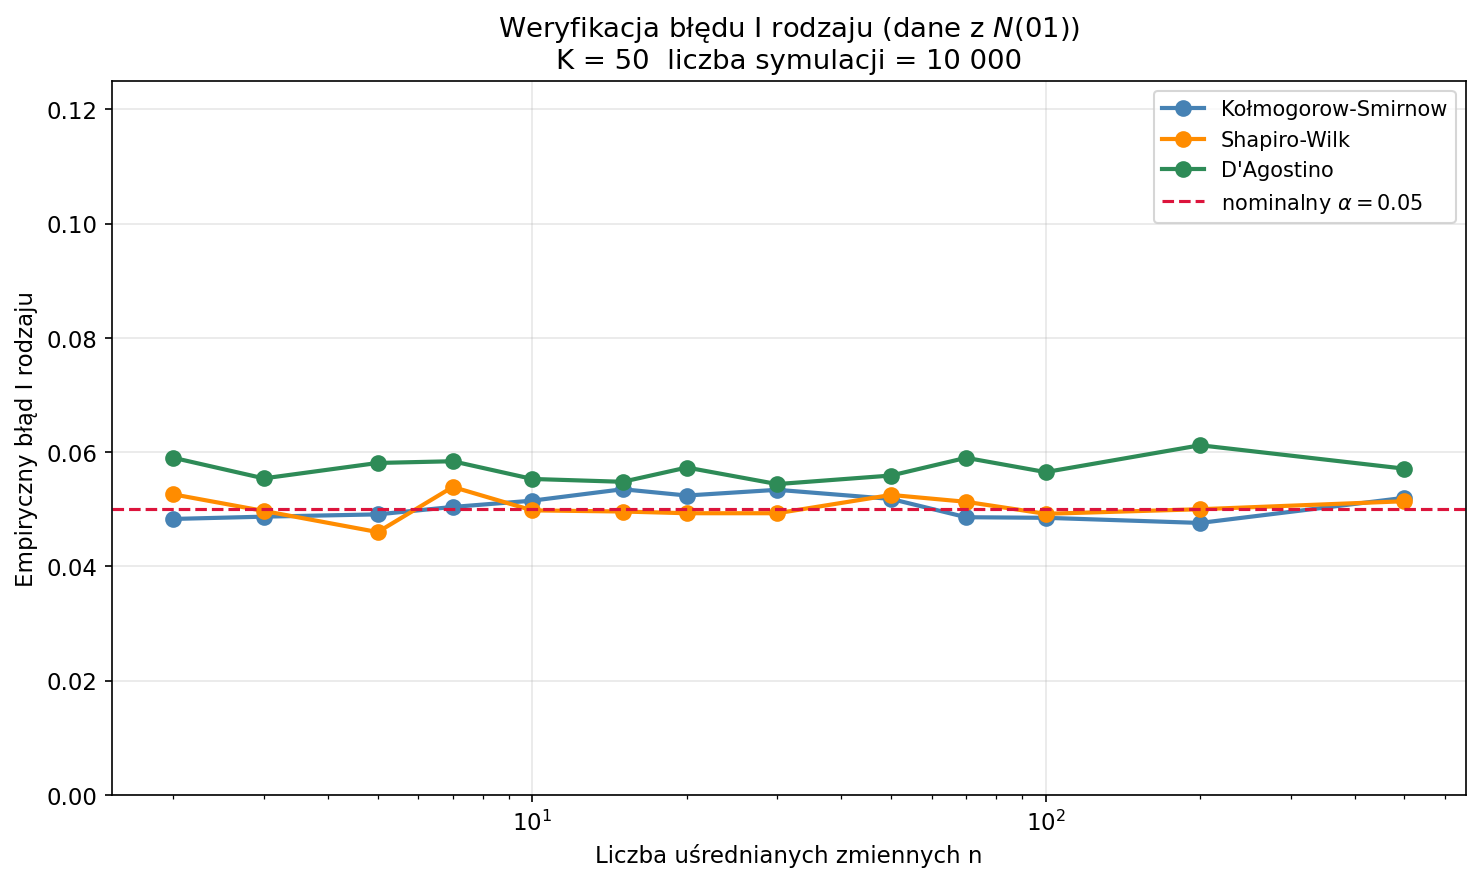
\includegraphics[width=\textwidth]{type_one_error.png}
    \caption{Weryfikacja błędu I rodzaju: empiryczna frakcja odrzuceń $H_0$ dla danych pochodzących z $N(0, 1)$ w funkcji $n$. Wszystkie krzywe oscylują w pobliżu nominalnego $\alpha = 0{,}05$.}
    \label{fig:type1}
\end{figure}

\subsubsection{Estymacja skośności i kurtozy nadmiarowej $\bar{X}_n$}

Dla pełnego zrozumienia, dlaczego test D'Agostino przestaje wykrywać odchylenia od normalności wraz ze wzrostem $n$, kluczowe są dwie wielkości, na których opiera się jego statystyka: skośność $g_1$ oraz kurtoza nadmiarowa $g_2$. Rysunek~\ref{fig:moments} przedstawia ich estymaty empiryczne wraz z krzywymi teoretycznymi $2/\sqrt{n}$ i $6/n$ właściwymi dla średniej z rozkładu $\mathrm{Exp}(1)$.

\begin{figure}[H]
    \centering
    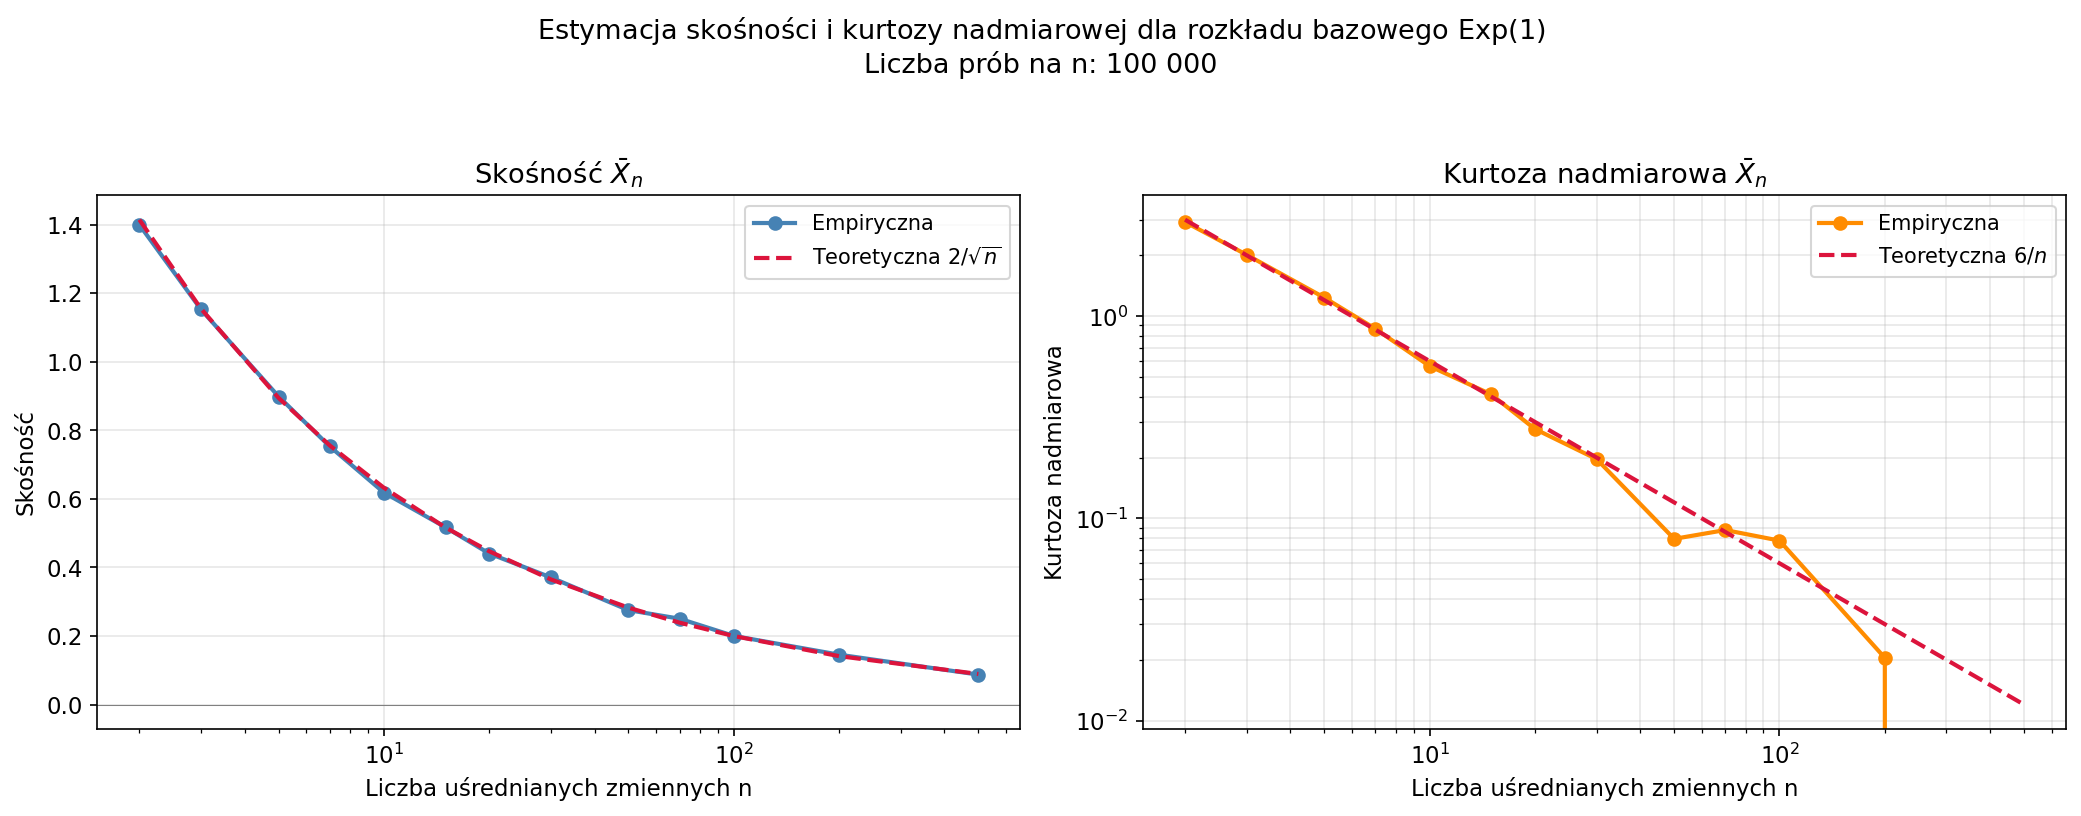
\includegraphics[width=\textwidth]{moments.png}
    \caption{Estymacja skośności (panel lewy) i kurtozy nadmiarowej (panel prawy) średniej $\bar{X}_n$ z rozkładu $\mathrm{Exp}(1)$. Punkty - wartości empiryczne (po $100\,000$ realizacji $\bar{X}_n$ dla każdego $n$); linie przerywane - teoretyczne $2/\sqrt{n}$ oraz $6/n$.}
    \label{fig:moments}
\end{figure}

Lewy panel pokazuje skośność. Punkty empiryczne pokrywają się z krzywą $2/\sqrt{n}$ z dokładnością odpowiadającą szumowi Monte Carlo - dla $n = 2$ wartość empiryczna wynosi $1{,}40$ przy teoretycznej $1{,}41$, dla $n = 30$ jest to $0{,}37$ wobec $0{,}37$, a dla $n = 500$ empiryczna skośność spada do $0{,}09$, w pełnej zgodzie z teorią. Prawy panel, w skali logarytmicznej na obu osiach, ilustruje analogiczne zachowanie kurtozy nadmiarowej: empiryczne wartości układają się wzdłuż linii prostej o nachyleniu odpowiadającym $1/n$. Dla największych $n$ punkty zaczynają nieznacznie odbiegać od linii teoretycznej - jest to efekt rosnącego względnego błędu estymatora kurtozy, gdy szacowana wartość zbliża się do zera (przy $n = 500$ teoretyczna kurtoza nadmiarowa wynosi $0{,}012$, więc nawet niewielka odchyłka empiryczna staje się widoczna w skali logarytmicznej).

Pełne wartości liczbowe zebrano w tabeli~\ref{tab:moments}.

\begin{table}[H]
    \centering
    \caption{Skośność i kurtoza nadmiarowa średniej $\bar{X}_n$ z rozkładu $\mathrm{Exp}(1)$: empiryczne wartości z $100\,000$ realizacji dla każdego $n$ i krzywe teoretyczne.}
    \label{tab:moments}
    \begin{tabular}{r|rr|rr}
\toprule
 & \multicolumn{2}{c|}{Skośność} & \multicolumn{2}{c}{Kurtoza nadmiarowa} \\
$n$ & empiryczna & teoretyczna $2/\sqrt{n}$ & empiryczna & teoretyczna $6/n$ \\
\midrule
2 & 1.3993 & 1.4142 & 2.9220 & 3.0000 \\
3 & 1.1525 & 1.1547 & 2.0117 & 2.0000 \\
5 & 0.8986 & 0.8944 & 1.2356 & 1.2000 \\
7 & 0.7531 & 0.7559 & 0.8661 & 0.8571 \\
10 & 0.6184 & 0.6325 & 0.5663 & 0.6000 \\
15 & 0.5170 & 0.5164 & 0.4103 & 0.4000 \\
20 & 0.4407 & 0.4472 & 0.2767 & 0.3000 \\
30 & 0.3710 & 0.3651 & 0.1966 & 0.2000 \\
50 & 0.2755 & 0.2828 & 0.0792 & 0.1200 \\
70 & 0.2506 & 0.2390 & 0.0876 & 0.0857 \\
100 & 0.2004 & 0.2000 & 0.0777 & 0.0600 \\
200 & 0.1456 & 0.1414 & 0.0204 & 0.0300 \\
500 & 0.0875 & 0.0894 & -0.0016 & 0.0120 \\
\bottomrule
\end{tabular}

\end{table}

\subsection{Interpretacja wyników i wnioski}

Wyniki symulacji prowadzą do kilku spójnych obserwacji, które łącznie odpowiadają na pytanie postawione w treści zadania.

Najwyższą moc w analizowanym przypadku wykazuje test Shapiro-Wilka. Jego przewaga jest widoczna w całym zakresie $n$ i wynika z konstrukcji statystyki: porównanie kombinacji liniowej statystyk pozycyjnych z wariancją próby jest czułe zarówno na asymetrię, jak i na ciężkie ogony rozkładu, a niewielkie $K$ (rzędu kilkudziesięciu) jest dla niego korzystne. Tuż za nim plasuje się test D'Agostino, który również daje wysoką moc dla małych $n$, lecz pozostaje konsekwentnie nieco słabszy od Shapiro-Wilka. Jego siła zależy bezpośrednio od skośności i kurtozy nadmiarowej $\bar{X}_n$: dla $n = 2$ skośność wynosi około $1{,}41$, a kurtoza $3$, więc test wyraźnie identyfikuje obie nieregularności. Dla $n = 50$ skośność spada do $0{,}28$, a kurtoza do $0{,}12$ - wartości te są już na tyle blisko zera, że statystyka $K^2$ rzadko przekracza wartość krytyczną i moc testu zbliża się do $\alpha$.

Test Kołmogorowa-Smirnowa wypada zdecydowanie najsłabiej. Wynika to z natury jego statystyki: maksymalna różnica między dystrybuantą empiryczną a dystrybuantą referencyjną jest miarą globalną i zwykle nieczułą na lokalne odchylenia w ogonach, które najmocniej różnicują rozkład $\bar{X}_n$ od normalnego. Test ten ma dodatkowo strukturalną wadę dla problemu testowania normalności - dla typowych zastosowań wymaga znajomości parametrów rozkładu albo specjalnej poprawki Lillieforsa; w niniejszej pracy zastosowano standaryzację z parametrami teoretycznymi $\mu$ i $\sigma$, co eliminuje konserwatyzm wynikający z estymacji parametrów z próby, lecz nie zmienia zasadniczo charakterystyki testu. Jego moc na poziomie $0{,}24$ przy $n = 2$ jest najgorszym wynikiem spośród wszystkich trzech metod, a dla $n \geq 30$ test ten działa praktycznie jak losowe odrzucenie z prawdopodobieństwem $\alpha$.

Estymacja skośności i kurtozy nadmiarowej bezpośrednio wyjaśnia kształt krzywej mocy testu D'Agostino. Tempo spadku tych wielkości (proporcjonalnie do $1/\sqrt{n}$ oraz $1/n$) odpowiada tempu zaniku mocy widocznemu na rysunku~\ref{fig:power}, co potwierdza, że test ten działa zgodnie z założeniami konstrukcyjnymi. Bardzo dobra zgodność wartości empirycznych z teorią dla rozkładu $\mathrm{Exp}(1)$ stanowi również silne potwierdzenie poprawności symulacji oraz precyzji estymatorów momentów.

Z punktu widzenia zastosowań praktycznych można sformułować następujący wniosek. W przypadku testowania normalności średniej arytmetycznej zmiennych skośnych przy umiarkowanej liczności próby $K$ (kilkadziesiąt obserwacji) najsensowniejszym wyborem jest test Shapiro-Wilka. Test D'Agostino stanowi rozsądną alternatywę, gdy chce się jednocześnie diagnozować, czy odchylenie od normalności wynika ze skośności, czy z grubości ogonów - wynik testu można wtedy uzupełnić bezpośrednią inspekcją wartości skośności i kurtozy. Testu Kołmogorowa-Smirnowa nie należy stosować jako podstawowego narzędzia do testowania normalności - jego moc jest znacząco niższa niż konkurencyjnych testów dedykowanych temu problemowi.

Wreszcie, niezależnie od użytego testu, wraz ze wzrostem $n$ wszystkie krzywe mocy zbiegają do poziomu istotności $\alpha = 0{,}05$. Oznacza to, że dla wystarczająco dużej liczby uśrednianych zmiennych żaden ze stosowanych testów nie potrafi już wykryć odchylenia $\bar{X}_n$ od rozkładu normalnego - rozkład ten staje się praktycznie nieodróżnialny od normalnego, co stanowi tezę Centralnego Twierdzenia Granicznego.

\section{Problem 2 - odbiornik znanego sygnału}

\subsection{Metoda rozwiązania problemu}

Zadanie polega na zaprojektowaniu algorytmu detekcji, który w odebranym sygnale $x(i)$, $i = 1, \dots, N$ rozpoznaje obecność ukrytego, ustalonego z góry kodu pseudoszumowego $s(i) \in \{-1, +1\}$ zatopionego w białym szumie gaussowskim $w(i) \sim \mathcal{N}(0, \sigma^2)$. Pomijając całą warstwę radiową (częstotliwość nośna, dobór anten, układy RF, synchronizacja) oraz przetwarzanie sygnału do postaci cyfrowej, ograniczamy się do dyskretnego problemu testowania dwóch prostych hipotez:
\begin{align}
    H_0 \!:& \quad x(i) = w(i), \\
    H_1 \!:& \quad x(i) = A\,s(i) + w(i),
\end{align}
gdzie $A$ jest nieznaną, dodatnią amplitudą sygnału. Poziom istotności testu odpowiada prawdopodobieństwu fałszywego alarmu i powinien być bardzo niski - w analizie rozważano wartości $\alpha \in \{10^{-2}, 10^{-3}, 10^{-4}, 10^{-6}\}$.

Optymalny test wynika bezpośrednio z lematu Neymana-Pearsona. Próbki $x(i)$ nie mają identycznego rozkładu, lecz są niezależne, a ich łączna funkcja wiarygodności pod każdą z hipotez ma postać:
\begin{align}
    L_0(\mathbf{x}) &= \prod_{i=1}^{N} \frac{1}{\sqrt{2\pi\sigma^2}} \exp\!\left(-\frac{x(i)^2}{2\sigma^2}\right), \\
    L_1(\mathbf{x}; A) &= \prod_{i=1}^{N} \frac{1}{\sqrt{2\pi\sigma^2}} \exp\!\left(-\frac{(x(i) - A s(i))^2}{2\sigma^2}\right).
\end{align}
Iloraz wiarygodności po skróceniu wspólnych czynników i wykorzystaniu tożsamości $\sum_i s(i)^2 = N$ daje:
\begin{equation}
    \log \frac{L_1}{L_0} = \frac{A}{\sigma^2} \sum_{i=1}^{N} s(i) x(i) - \frac{A^2 N}{2\sigma^2}.
\end{equation}
Drugi człon nie zależy od danych, więc po zastosowaniu progowania na ilorazie wiarygodności decyzja sprowadza się do porównania pojedynczej statystyki
\begin{equation}
    T = \sum_{i=1}^{N} s(i)\,x(i)
    \label{eq:T}
\end{equation}
z progiem $\tau$. Statystyka $T$ jest zatem statystyką dostateczną dla problemu detekcji, a dla każdego $A > 0$ uzyskany test jest jednostajnie najmocniejszy w klasie testów o ustalonym poziomie istotności. W praktyce statystyka ta odpowiada operacji korelacji sygnału odebranego ze znanym kodem, czyli klasycznemu filtrowi dopasowanemu (matched filter).

Rozkład statystyki testowej jest pod obiema hipotezami gaussowski, ponieważ $T$ jest kombinacją liniową zmiennych normalnych. Bezpośrednie obliczenie wartości oczekiwanej i wariancji daje:
\begin{align}
    T \mid H_0 &\sim \mathcal{N}(0, \sigma^2 N), \\
    T \mid H_1 &\sim \mathcal{N}(A N, \sigma^2 N).
\end{align}
Próg dobiera się tak, aby prawdopodobieństwo fałszywego alarmu wynosiło dokładnie $\alpha$:
\begin{equation}
    \tau = z_{1-\alpha} \, \sigma \sqrt{N},
\end{equation}
gdzie $z_{1-\alpha}$ to kwantyl rzędu $1-\alpha$ rozkładu $\mathcal{N}(0,1)$. Moc testu, czyli prawdopodobieństwo poprawnej detekcji, wyraża się wzorem:
\begin{equation}
    P_D = \Pr(T > \tau \mid H_1) = 1 - \Phi\!\left(z_{1-\alpha} - \frac{A\sqrt{N}}{\sigma}\right) = \Phi(d - z_{1-\alpha}),
    \label{eq:power}
\end{equation}
gdzie $\Phi$ oznacza dystrybuantę rozkładu standardowego normalnego, a wielkość
\begin{equation}
    d = \frac{A\sqrt{N}}{\sigma}
    \label{eq:d}
\end{equation}
nazywana będzie dalej \emph{efektywnym stosunkiem sygnału do szumu}. To kluczowy parametr układu - moc detekcji zależy od $A$, $\sigma$ i $N$ wyłącznie poprzez ich kombinację $d$. Wynika z tego natychmiast efekt zwany \emph{processing gain}: dwukrotne wydłużenie sygnału kompensuje obniżenie amplitudy o czynnik $\sqrt{2}$ albo wzrost odchylenia standardowego szumu o ten sam czynnik. Inaczej mówiąc, można wykryć dowolnie słaby sygnał, jeśli tylko dostatecznie długo można obserwować jego znaną strukturę.

Symulacje Monte Carlo zrealizowano w języku Python z wykorzystaniem bibliotek \texttt{numpy} oraz \texttt{scipy.stats}. Dla każdego zestawu parametrów $(N, A, \sigma, \alpha)$ wylosowano kod $s$ ze stałym ziarnem generatora (rozłożenia $\pm 1$ z równym prawdopodobieństwem), a następnie wygenerowano po $50\,000$ niezależnych realizacji szumu pod obiema hipotezami. Empiryczne wartości prawdopodobieństw $P_D$ i $P_{FA}$ obliczono jako frakcję przekroczeń progu. Wszystkie generatory liczb pseudolosowych zainicjalizowano ziarnami pochodnymi od stałej $\mathrm{SEED} = 42$, co zapewnia powtarzalność wyników.

\subsection{Wyniki}

\subsubsection{Rozkład statystyki testu i weryfikacja teorii}

Punktem wyjścia analizy jest sprawdzenie, czy rozkład statystyki testowej $T$ pod obiema hipotezami rzeczywiście pokrywa się z formułami teoretycznymi. Rysunek~\ref{fig:test_stat} przedstawia histogramy gęstości $T$ uzyskane z $200\,000$ realizacji dla wybranego zestawu parametrów ($N = 256$, $A = 0{,}3$, $\sigma = 1$). Pod $H_0$ histogram jest symetryczny wokół zera o rozrzucie $\sigma\sqrt{N} \approx 16$, pod $H_1$ jego środek przesuwa się o $AN = 76{,}8$, lecz rozrzut pozostaje identyczny. Naniesione krzywe teoretyczne $\mathcal{N}(0, \sigma^2 N)$ oraz $\mathcal{N}(AN, \sigma^2 N)$ pokrywają histogramy z dokładnością nieodróżnialną gołym okiem. Czerwona pionowa linia oznacza próg $\tau$ dla $\alpha = 10^{-3}$, który oddziela praktycznie cały rozkład pod $H_0$ od większości masy rozkładu pod $H_1$, ilustrując mechanizm detekcji.

\begin{figure}[H]
    \centering
    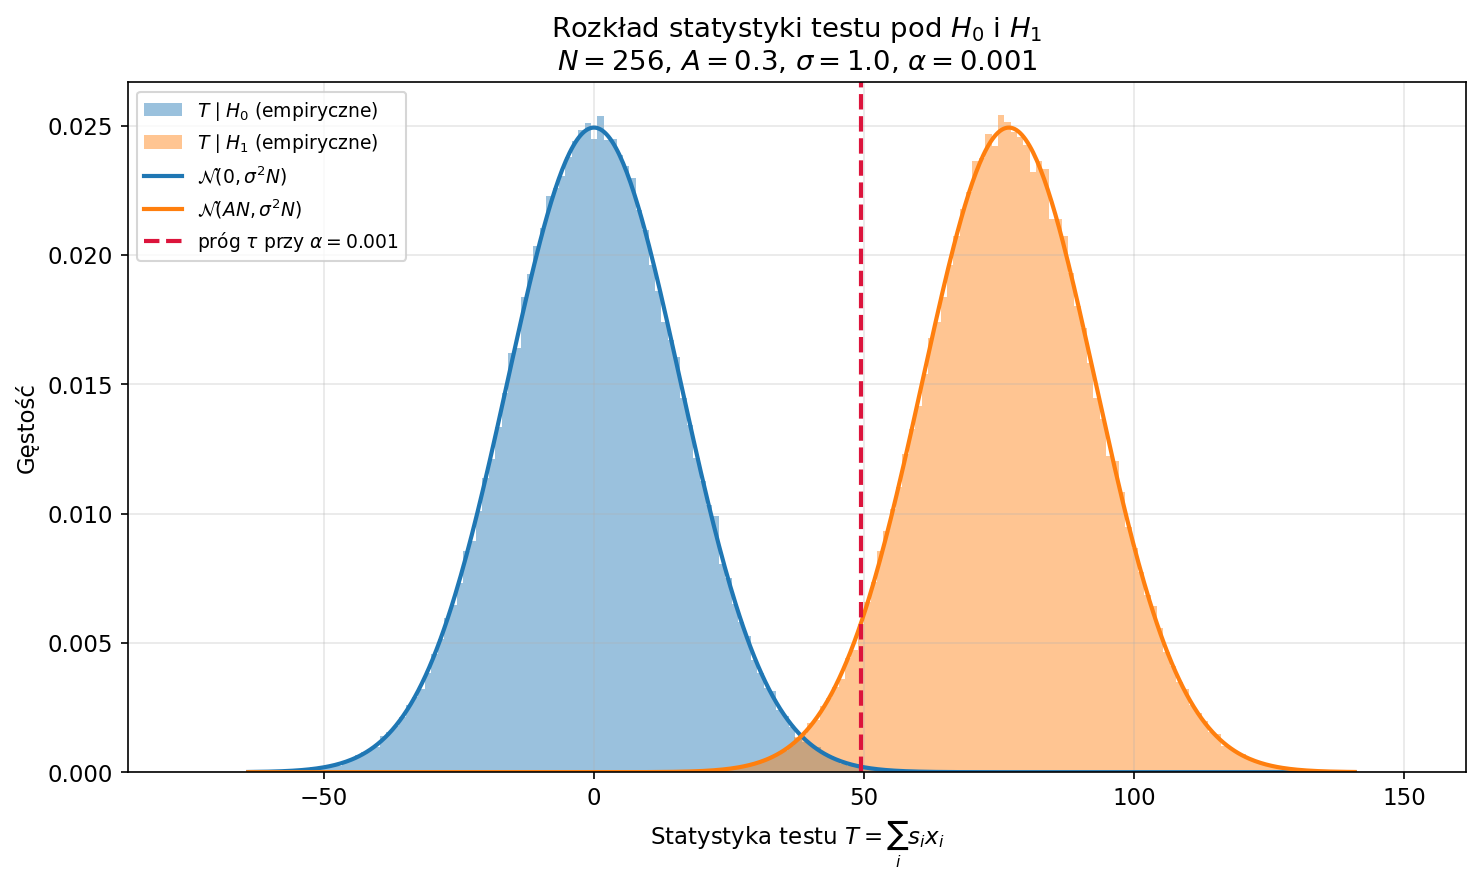
\includegraphics[width=\textwidth]{test_statistic.png}
    \caption{Rozkład statystyki testu $T = \sum_i s(i) x(i)$ pod hipotezami $H_0$ i $H_1$ wraz z teoretycznymi krzywymi gęstości oraz progiem decyzyjnym przy $\alpha = 10^{-3}$.}
    \label{fig:test_stat}
\end{figure}

Tabela~\ref{tab:verification} zestawia teoretyczne i empiryczne wartości mocy detekcji oraz empiryczny rozmiar testu dla siedmiu reprezentatywnych konfiguracji $(N, A, \alpha)$. We wszystkich przypadkach wartości empiryczne odbiegają od teoretycznych o nie więcej niż dwie cyfry znaczące, co w pełni mieści się w błędzie Monte Carlo dla $50\,000$ symulacji. Podobnie empiryczne prawdopodobieństwo fałszywego alarmu pozostaje praktycznie identyczne z nominalnym $\alpha$, co potwierdza poprawność wyboru progu.

\begin{table}[H]
    \centering
    \caption{Weryfikacja teoretycznych wzorów na moc detekcji i poziom fałszywego alarmu - empiryczne wartości z $50\,000$ symulacji Monte Carlo dla wybranych konfiguracji parametrów ($\sigma = 1$).}
    \label{tab:verification}
    \begin{tabular}{rrrrrr}
\toprule
$N$ & $A$ & $\alpha$ & $P_D$ teoria & $P_D$ empir. & $P_{FA}$ empir. \\
\midrule
256 & 0.10 & 1e-02 & 0.2338 & 0.2344 & 0.0094 \\
256 & 0.20 & 1e-02 & 0.8088 & 0.8077 & 0.0103 \\
256 & 0.30 & 1e-03 & 0.9563 & 0.9576 & 0.0010 \\
1024 & 0.05 & 1e-03 & 0.0681 & 0.0669 & 0.0011 \\
1024 & 0.10 & 1e-03 & 0.5437 & 0.5448 & 0.0013 \\
4096 & 0.03 & 1e-03 & 0.1210 & 0.1202 & 0.0010 \\
4096 & 0.05 & 1e-02 & 0.8088 & 0.8092 & 0.0104 \\
\bottomrule
\end{tabular}

\end{table}

\subsubsection{Wpływ amplitudy, długości sygnału i poziomu szumu}

Wzór~\eqref{eq:power} przewiduje, że moc testu zależy od trzech parametrów $A$, $N$, $\sigma$ jedynie poprzez efektywny stosunek $d = A\sqrt{N}/\sigma$. Aby zilustrować rolę każdego z nich osobno, kolejne trzy rysunki pokazują przekroje tej zależności, w których jeden parametr jest zmieniany, a pozostałe pozostają stałe.

Rysunek~\ref{fig:power_A} przedstawia moc detekcji w funkcji amplitudy $A$ przy ustalonym $\sigma = 1$ i $\alpha = 10^{-3}$, dla pięciu wartości $N \in \{16, 64, 256, 1024, 4096\}$. Wszystkie krzywe mają charakterystyczny kształt sigmoidalny, gwałtownie przechodząc od $P_D \approx \alpha$ dla małych $A$ do $P_D \approx 1$ dla dużych. Punkt przegięcia każdej krzywej (mocy 0{,}5) przypada na $A \approx z_{1-\alpha} \sigma / \sqrt{N}$, czyli skaluje się jak $1/\sqrt{N}$. Praktyczna konsekwencja jest taka, że czterokrotne wydłużenie sygnału obniża wymaganą amplitudę detekcji dwukrotnie.

\begin{figure}[H]
    \centering
    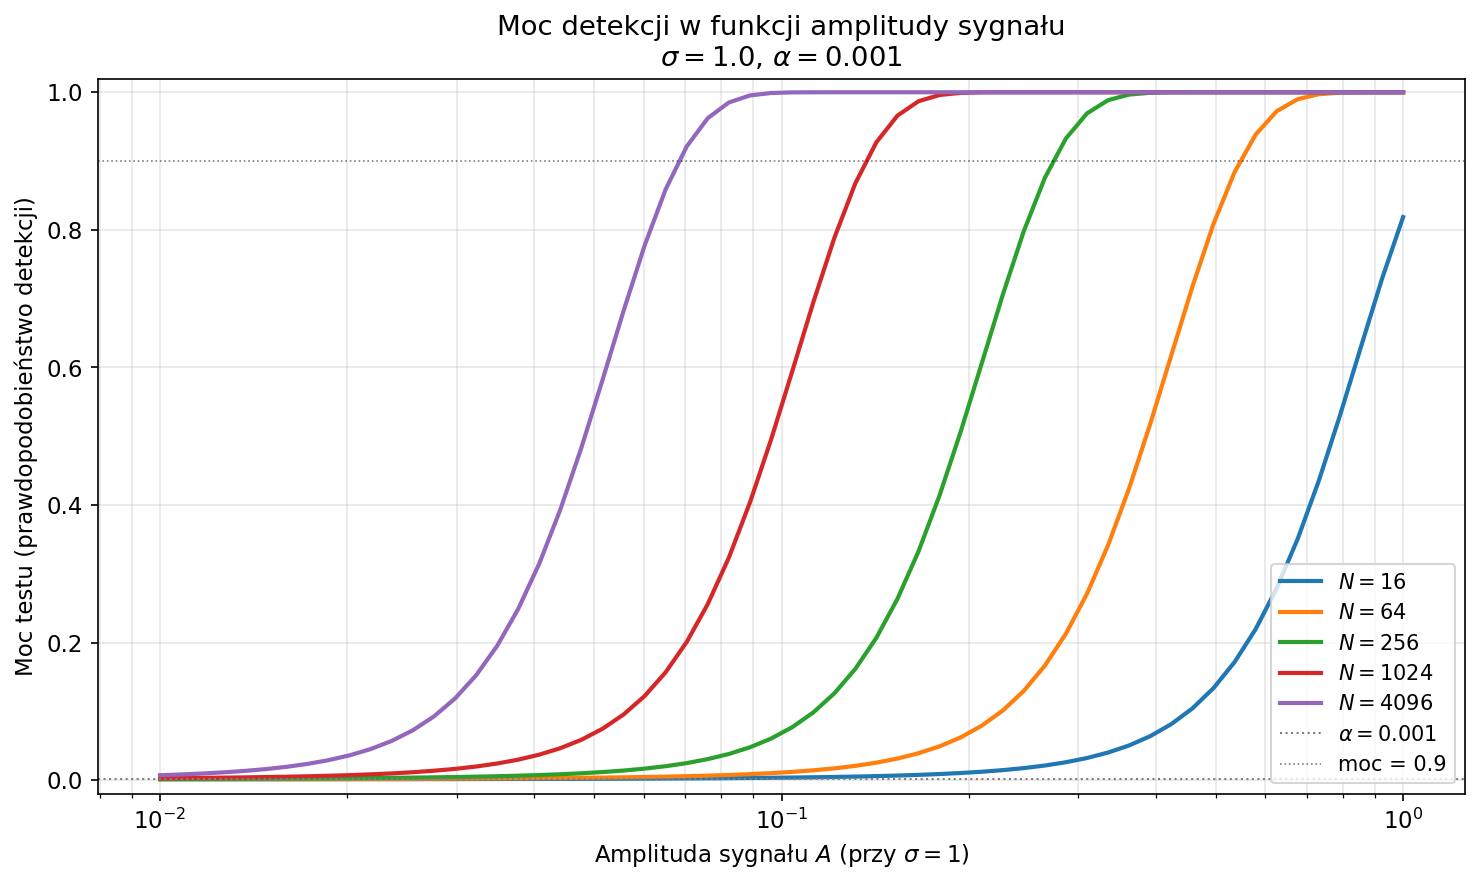
\includegraphics[width=\textwidth]{power_vs_amplitude.png}
    \caption{Moc detekcji w funkcji amplitudy sygnału $A$ dla różnych długości $N$ przy stałym $\sigma = 1$, $\alpha = 10^{-3}$.}
    \label{fig:power_A}
\end{figure}

Rysunek~\ref{fig:power_N} pokazuje to samo zjawisko z innej perspektywy - moc w funkcji długości sygnału $N$ przy ustalonych wartościach stosunku $A/\sigma \in \{0{,}05; 0{,}1; 0{,}2; 0{,}5; 1{,}0\}$. Krzywe są symetrycznie przesunięte względem siebie w skali logarytmicznej osi $N$: aby uzyskać tę samą moc detekcji, dwukrotne zmniejszenie amplitudy wymaga czterokrotnego wydłużenia sygnału. Dla $A = 0{,}05\sigma$ osiągnięcie mocy 0{,}9 wymaga $N$ rzędu $5000$ próbek, podczas gdy dla $A = \sigma$ wystarczy zaledwie kilkanaście próbek.

\begin{figure}[H]
    \centering
    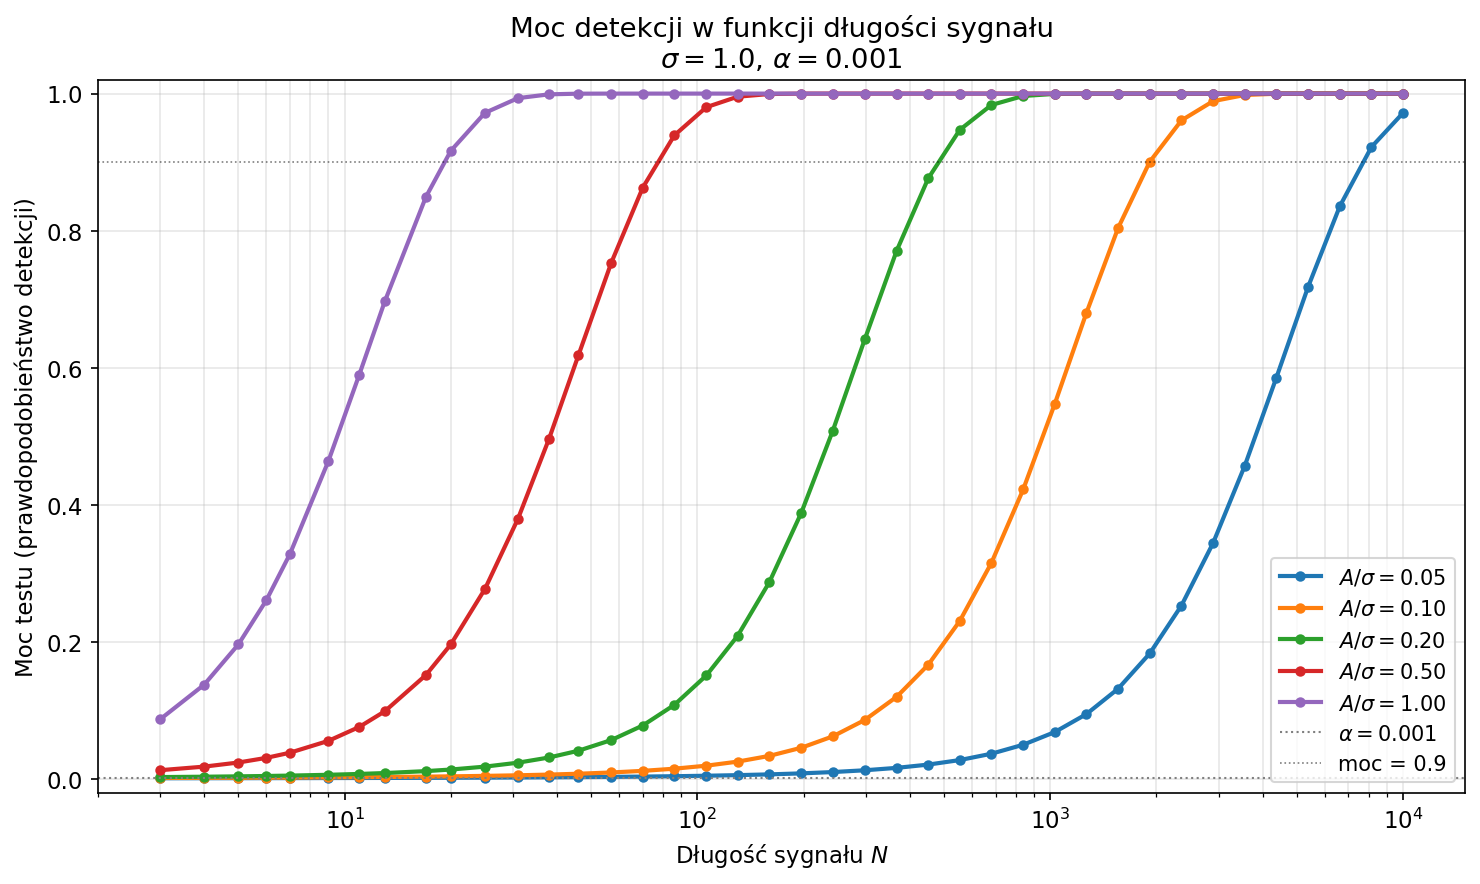
\includegraphics[width=\textwidth]{power_vs_n.png}
    \caption{Moc detekcji w funkcji długości sygnału $N$ dla różnych stosunków $A/\sigma$ przy $\alpha = 10^{-3}$.}
    \label{fig:power_N}
\end{figure}

Trzecim parametrem analizowanym osobno jest odchylenie standardowe szumu $\sigma$. Rysunek~\ref{fig:power_sigma} pokazuje moc detekcji jako funkcję $\sigma$ dla pięciu kombinacji $(A, N)$. Zgodnie z formułą~\eqref{eq:power} każda krzywa monotonicznie maleje wraz ze wzrostem poziomu szumu, dążąc do wartości $\alpha$ dla bardzo dużego $\sigma$. Kombinacje, które dają identyczny iloczyn $A\sqrt{N}$, prowadzą do krzywych o tym samym kształcie, jedynie przesuniętych wzdłuż osi $\sigma$. Konfiguracje $A = 0{,}3$, $N = 1024$ oraz $A = 0{,}1$, $N = 4096$ na rysunku wyglądają prawie identycznie, gdyż obie odpowiadają tej samej wartości $A\sqrt{N} \approx 9{,}6$. Dla pierwszej z nich detektor utrzymuje moc 0{,}9 aż do $\sigma \approx 2{,}5$, podczas gdy konfiguracja $A = 0{,}3$, $N = 256$ traci tę zdolność już dla $\sigma \approx 1{,}25$.

\begin{figure}[H]
    \centering
    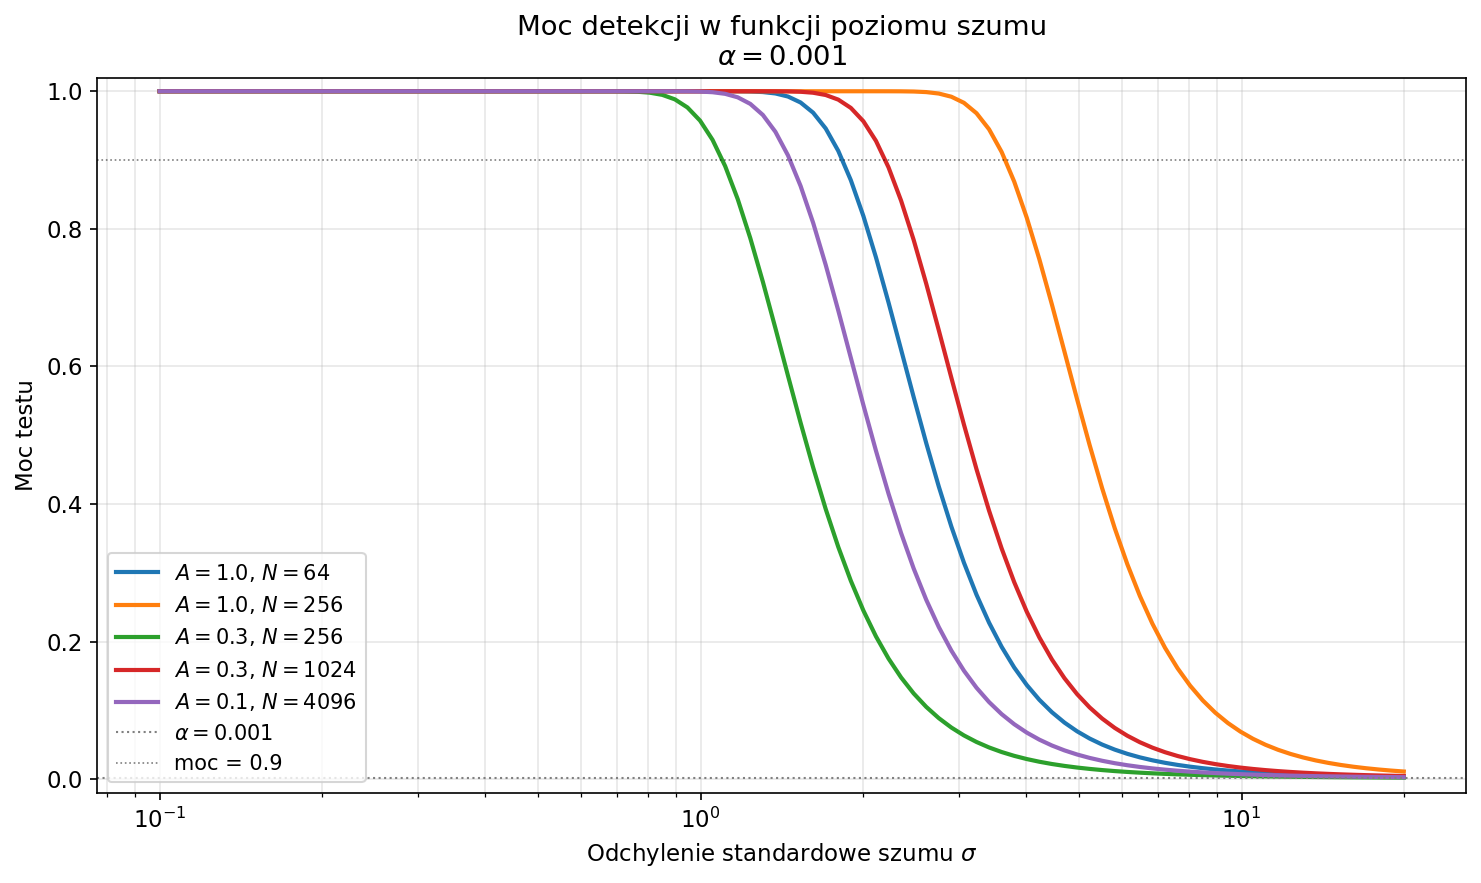
\includegraphics[width=\textwidth]{power_vs_sigma.png}
    \caption{Moc detekcji w funkcji odchylenia standardowego szumu $\sigma$ dla różnych kombinacji $(A, N)$ przy $\alpha = 10^{-3}$.}
    \label{fig:power_sigma}
\end{figure}

\subsubsection{Wpływ poziomu istotności i uniwersalne skalowanie}

Wymóg bardzo niskiego prawdopodobieństwa fałszywego alarmu, podany wprost w treści zadania, znacząco zmienia wymagania na sygnał. Rysunek~\ref{fig:power_alpha} pokazuje moc detekcji w funkcji $\alpha$ przy ustalonym $N = 256$ dla czterech wartości amplitudy. Dla każdej z nich obniżenie $\alpha$ o cztery rzędy wielkości (z $10^{-2}$ do $10^{-6}$) wymaga proporcjonalnie większego marginesu w efektywnym SNR. Przy $A = 0{,}5$ ($d = 8$) detektor utrzymuje moc bliską 1 nawet dla $\alpha = 10^{-8}$, natomiast przy $A = 0{,}1$ ($d = 1{,}6$) już dla $\alpha = 10^{-3}$ moc spada poniżej 30\%.

\begin{figure}[H]
    \centering
    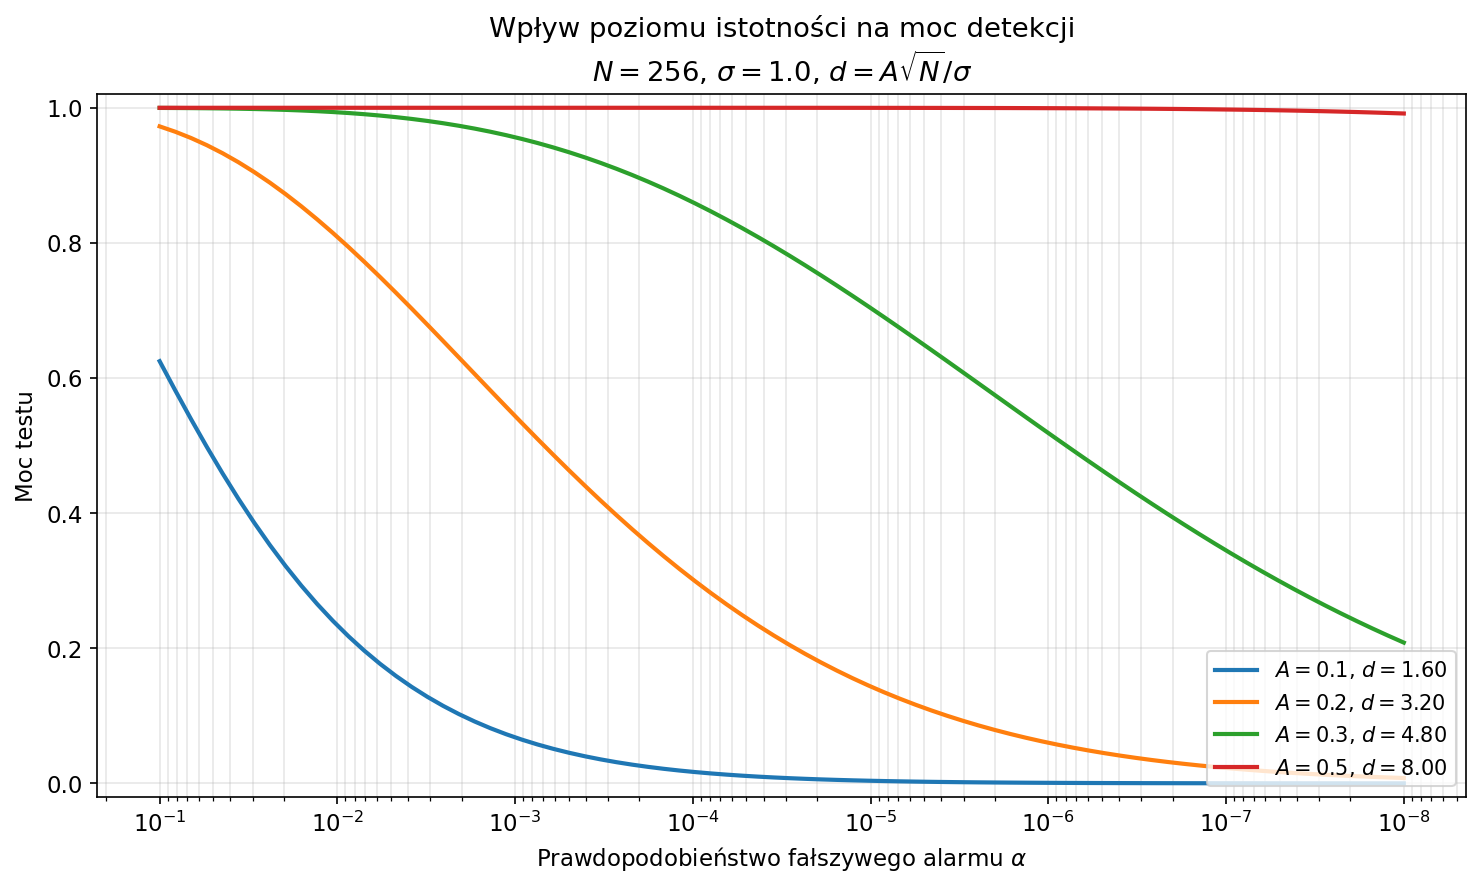
\includegraphics[width=\textwidth]{power_vs_alpha.png}
    \caption{Moc detekcji w funkcji prawdopodobieństwa fałszywego alarmu $\alpha$ dla różnych amplitud sygnału przy $N = 256$, $\sigma = 1$.}
    \label{fig:power_alpha}
\end{figure}

Trzy poprzednie rysunki można uznać za różne projekcje jednej fundamentalnej zależności. Rysunek~\ref{fig:gain} przedstawia tę zależność wprost - moc detekcji jako funkcję efektywnego SNR $d = A\sqrt{N}/\sigma$ dla czterech poziomów istotności. Każda krzywa jest przesuniętą kopią dystrybuanty rozkładu standardowego normalnego $\Phi(d - z_{1-\alpha})$, a wszystkie kombinacje $(A, N, \sigma)$ dające tę samą wartość $d$ leżą dokładnie na tej krzywej. Praktyczne progi detekcji są łatwo odczytywalne z wykresu - osiągnięcie mocy 0{,}9 wymaga $d \approx 4{,}1$ dla $\alpha = 10^{-3}$ oraz $d \approx 6{,}0$ dla $\alpha = 10^{-6}$.

\begin{figure}[H]
    \centering
    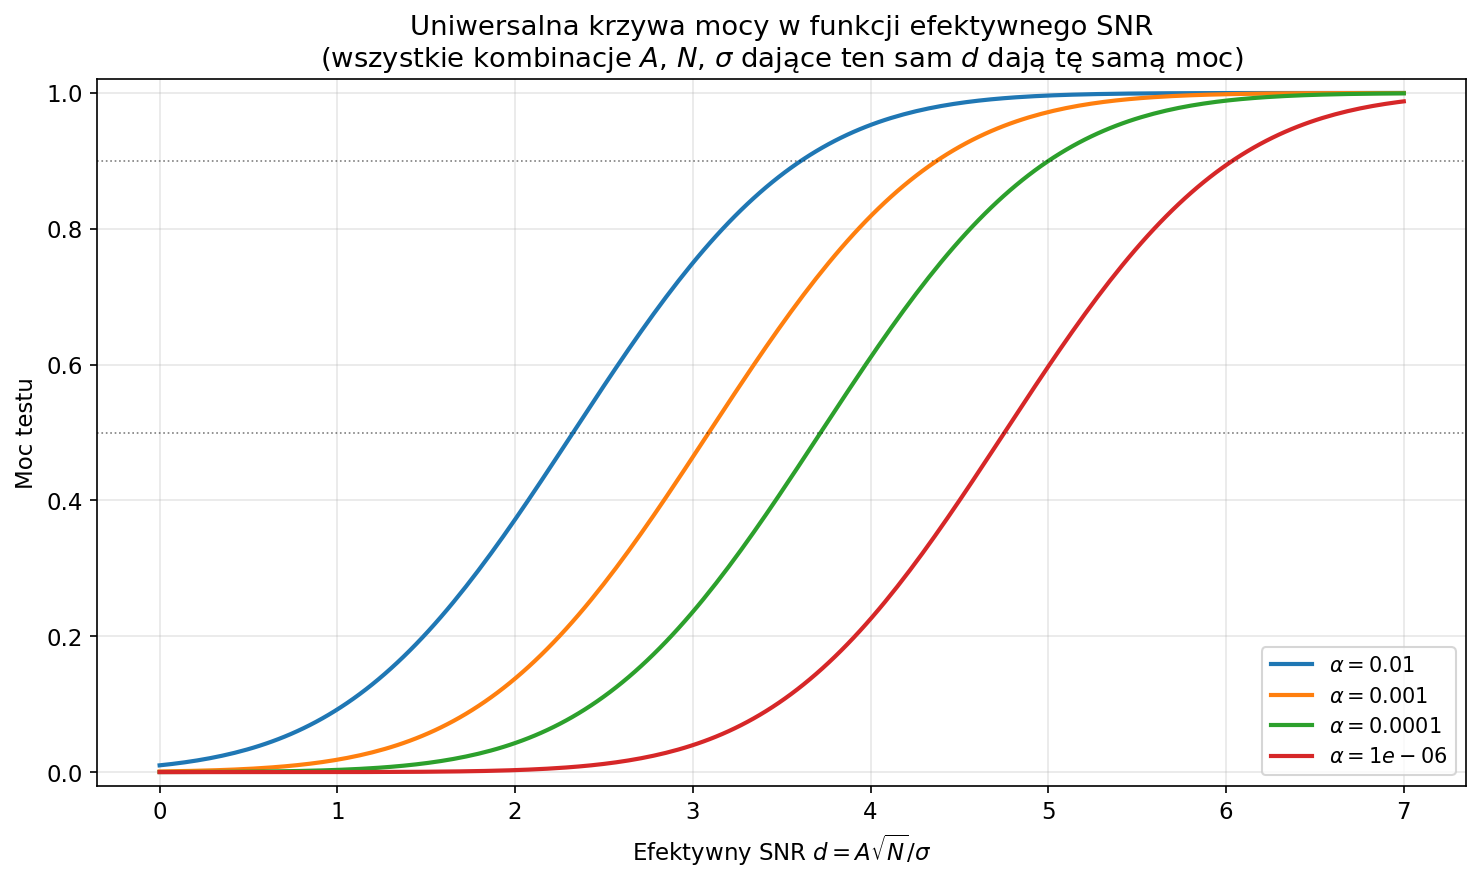
\includegraphics[width=\textwidth]{processing_gain.png}
    \caption{Uniwersalna krzywa mocy detekcji jako funkcja efektywnego stosunku sygnału do szumu $d = A\sqrt{N}/\sigma$ dla różnych poziomów istotności.}
    \label{fig:gain}
\end{figure}

Uzupełnieniem analizy są krzywe ROC (rysunek~\ref{fig:roc}), które dla pięciu wartości efektywnego SNR $d \in \{0{,}5;\, 1;\, 2;\, 3;\, 4\}$ pokazują pełen zakres możliwych kompromisów między prawdopodobieństwem detekcji a prawdopodobieństwem fałszywego alarmu. Dla $d = 0{,}5$ detektor pracuje niewiele lepiej od losowego, natomiast dla $d = 4$ krzywa jest tak blisko lewego górnego rogu wykresu, że przy $P_{FA} = 10^{-3}$ daje już $P_D > 0{,}97$, a przy $P_{FA} = 10^{-6}$ wciąż przekracza $0{,}75$.

\begin{figure}[H]
    \centering
    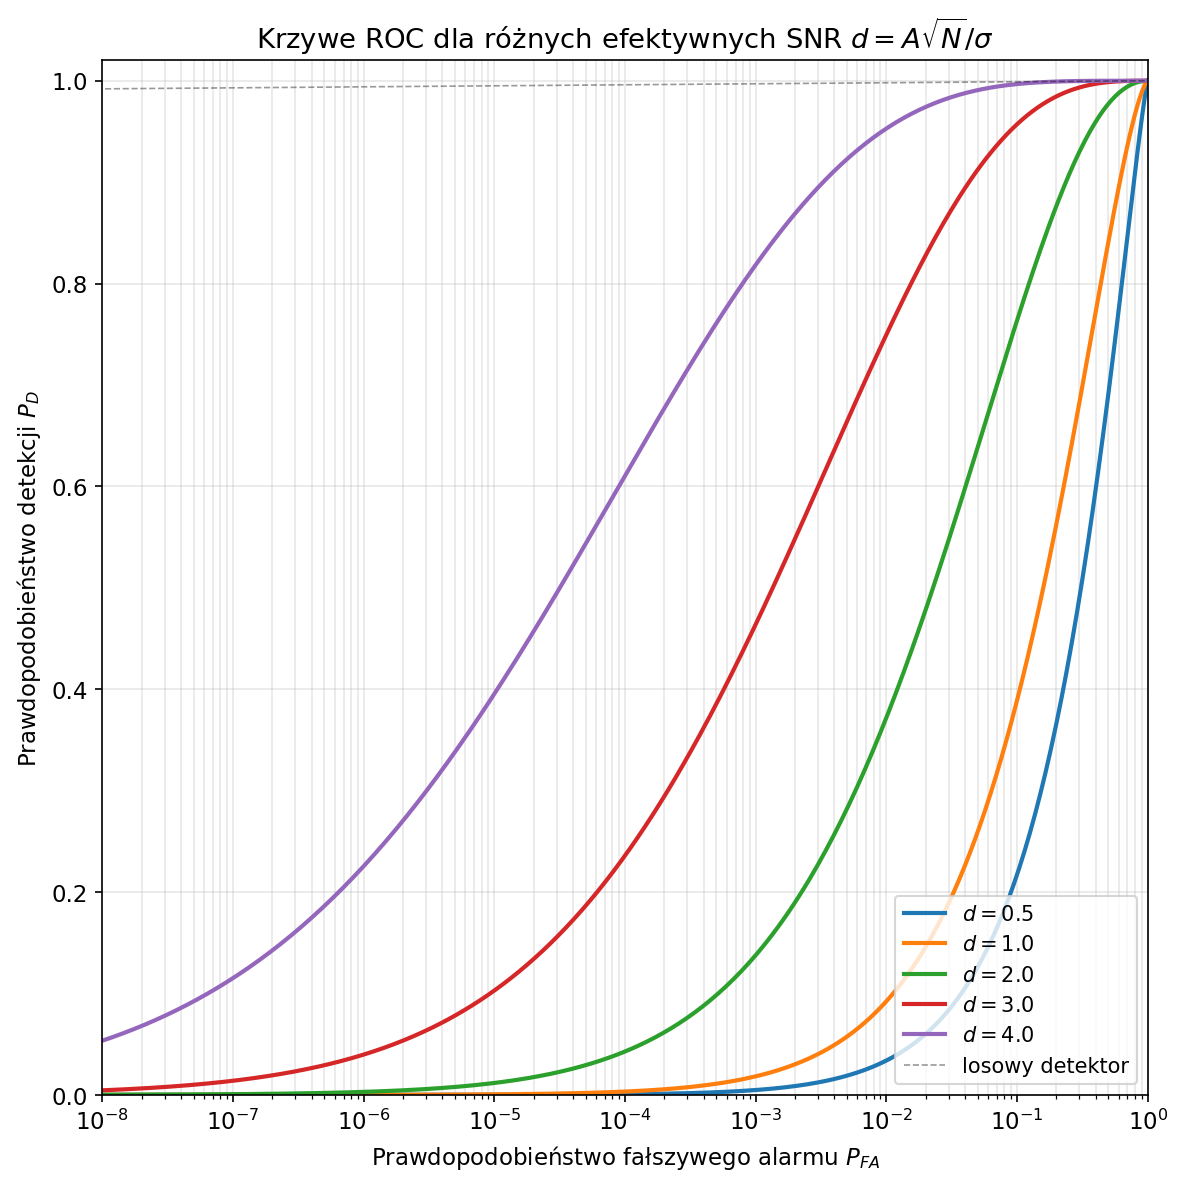
\includegraphics[width=0.85\textwidth]{roc.png}
    \caption{Krzywe ROC dla pięciu wartości efektywnego stosunku sygnału do szumu $d = A\sqrt{N}/\sigma$.}
    \label{fig:roc}
\end{figure}

\subsubsection{Detekcja sygnału bardzo słabego $A \ll \sigma$}

Najbardziej praktyczny aspekt tego zadania - detekcja sygnału o amplitudzie znacznie mniejszej od poziomu szumu - wynika bezpośrednio z formuły~\eqref{eq:d}. Jeśli ustalić docelową moc detekcji, to wymagana długość sygnału skaluje się jak $N \propto (\sigma/A)^2$. Rysunek~\ref{fig:weak} pokazuje krzywe mocy w funkcji $N$ dla czterech wartości amplitudy słabego sygnału w przedziale od $A = 0{,}01\sigma$ do $A = 0{,}3\sigma$. Liczby w legendzie podają długość sygnału potrzebną do osiągnięcia mocy 0{,}5 przy $\alpha = 10^{-3}$ - przy $A = 0{,}3\sigma$ wystarczy $N \approx 107$, przy $A = 0{,}1\sigma$ trzeba $N \approx 955$, przy $A = 0{,}03\sigma$ już ponad dziesięć tysięcy próbek, a przy $A = 0{,}01\sigma$ blisko sto tysięcy. Kwadratowe skalowanie tej liczby z odwrotnością stosunku $A/\sigma$ jest dobrze widoczne na osi logarytmicznej jako stała odległość między krzywymi.

\begin{figure}[H]
    \centering
    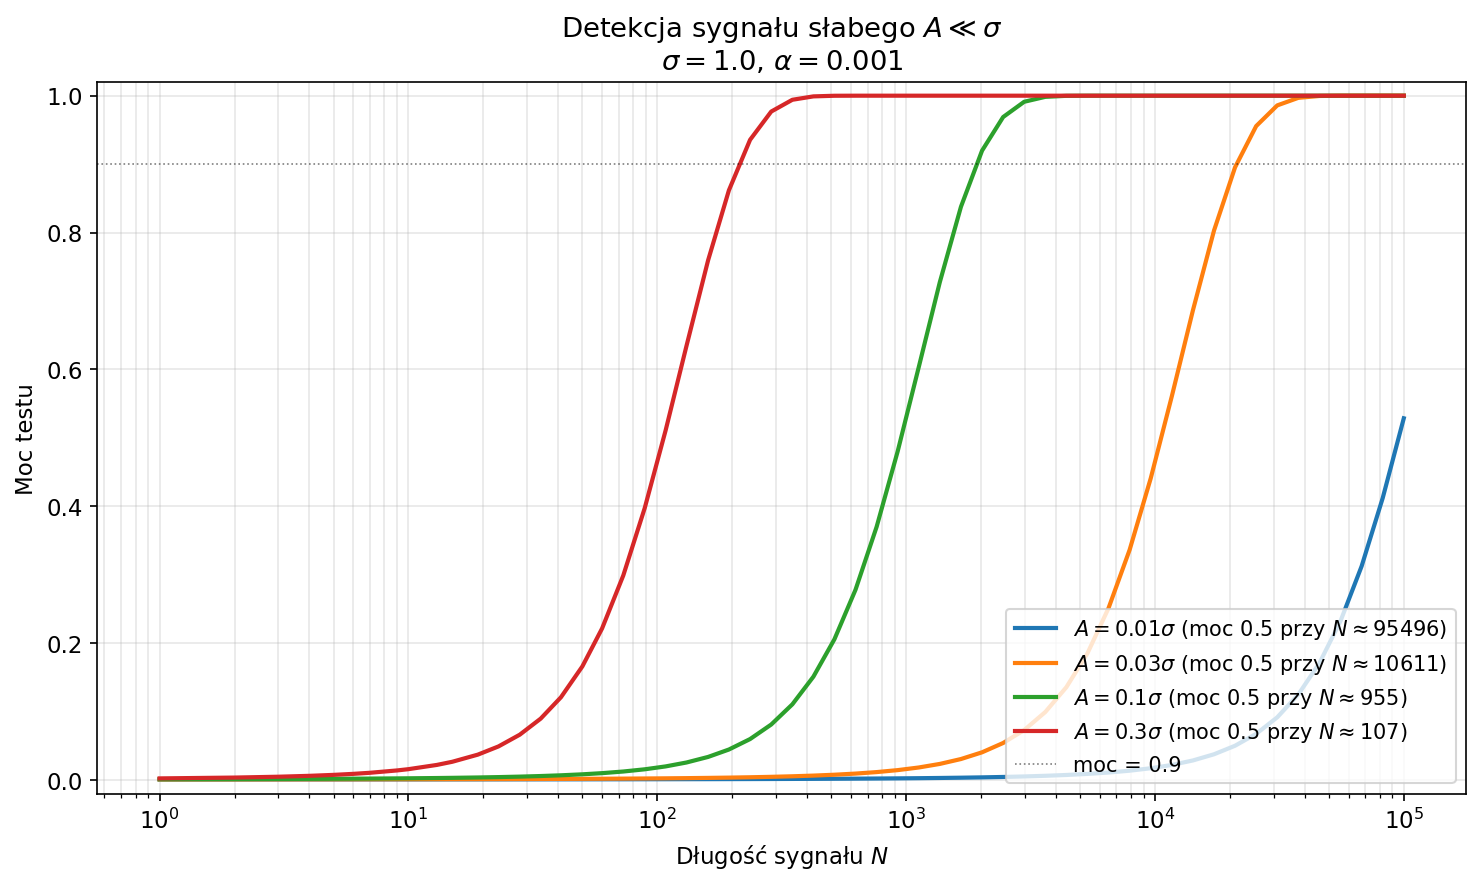
\includegraphics[width=\textwidth]{weak_signal.png}
    \caption{Detekcja sygnału słabego $A \ll \sigma$ - moc w funkcji długości sygnału $N$ dla czterech amplitud w zakresie $0{,}01\sigma$ do $0{,}3\sigma$ przy $\alpha = 10^{-3}$.}
    \label{fig:weak}
\end{figure}

Z punktu widzenia projektu systemu detekcji oznacza to, że nawet amplituda dwóch rzędów wielkości mniejsza od odchylenia szumu jest fundamentalnie wykrywalna - cena pozostaje jedynie w postaci czasu obserwacji, który rośnie kwadratowo wraz ze spadkiem amplitudy.

\subsection{Interpretacja wyników i wnioski}

Wszystkie uzyskane wyniki są wewnętrznie spójne i bezpośrednio wynikają z jednego centralnego wzoru~\eqref{eq:power}. Ich łączna interpretacja pozwala sformułować kilka praktycznych obserwacji.

Po pierwsze, optymalny detektor sygnału o znanej strukturze polega na jego skorelowaniu z odebranym sygnałem - jest to bezpośrednia konsekwencja lematu Neymana-Pearsona, a nie heurystyka. Statystyka $T = \sum_i s(i)\,x(i)$ jest sumą $N$ niezależnych zmiennych gaussowskich, dlatego ma rozkład normalny pod każdą z hipotez i pozwala na ścisłą, analityczną kontrolę poziomu fałszywego alarmu poprzez wybór progu $\tau = z_{1-\alpha}\sigma\sqrt{N}$.

Po drugie, kluczową miarą jakości detekcji jest pojedyncza wielkość, efektywny stosunek sygnału do szumu $d = A\sqrt{N}/\sigma$, łącząca wszystkie trzy parametry wymienione w treści zadania. Trzy oddzielne rysunki (\ref{fig:power_A}, \ref{fig:power_N} i \ref{fig:power_sigma}) różnią się jedynie wyborem osi poziomej, lecz każda krzywa na każdym z nich odpowiada określonej wartości $d$ - to wyjaśnia, dlaczego wszystkie projekcje składają się w jedną uniwersalną krzywą na rysunku~\ref{fig:gain}. Z tej obserwacji wynika praktyczna zasada projektowa: niedostatek w jednym parametrze można zawsze zrekompensować nadmiarem w innym, według reguły $A^2 N / \sigma^2 = \mathrm{const}$.

Po trzecie, detekcja sygnału znacznie słabszego od szumu nie napotyka żadnej fundamentalnej bariery - jak pokazuje rysunek~\ref{fig:weak}, nawet przy $A = 0{,}01\sigma$ wystarczająco długi sygnał pozwala uzyskać moc detekcji bliską jedności. Cena, jaką trzeba zapłacić, to kwadratowy wzrost długości sygnału względem odwrotności amplitudy. To właśnie dzięki tej zasadzie pseudoszumowy kod o długości $N$ rzędu kilku tysięcy próbek pozostaje praktycznie niewykrywalny dla osoby trzeciej, która nie zna $s(i)$, lecz jest pewnie wykrywany przez odbiorcę dysponującego dopasowanym filtrem.

Po czwarte, wymóg bardzo niskiego prawdopodobieństwa fałszywego alarmu (rysunek~\ref{fig:power_alpha}) zwiększa konieczny SNR jedynie logarytmicznie, ponieważ kwantyl $z_{1-\alpha}$ rośnie bardzo wolno wraz ze spadkiem $\alpha$. Przejście z $\alpha = 10^{-3}$ ($z_{1-\alpha} \approx 3{,}09$) do $\alpha = 10^{-6}$ ($z_{1-\alpha} \approx 4{,}75$) zwiększa wymagany efektywny SNR o niespełna dwa, co zwykle jest cenowo dostępne przez umiarkowane wydłużenie sygnału.

\subsection{Koncepcja systemu telekomunikacyjnego}

Sformułowany detektor stanowi w istocie odbiornik jednego bitu informacji - obecność sygnału alarmowego można utożsamić z bitem "1", brak alarmu z bitem "0". Ustalenie wartości krytycznej progu sprowadza się wtedy do problemu optymalizacji decyzji binarnej. W klasycznym podejściu Neymana-Pearsona, użytym powyżej, próg dobiera się tak, aby utrzymać zadany maksymalny koszt fałszywego alarmu, co odpowiada minimalizacji prawdopodobieństwa pominięcia sygnału przy ograniczeniu na $P_{FA}$. W podejściu bayesowskim, jeśli znane są prawdopodobieństwa apriori obu bitów $\pi_0$ i $\pi_1$ oraz koszty błędów obu rodzajów $c_{10}$ i $c_{01}$, optymalny próg minimalizuje średni oczekiwany koszt i wynosi $\tau^* = \sigma^2 / A \cdot \log\!\left(\pi_0 c_{10} / (\pi_1 c_{01})\right) + AN/2$. W symetrycznym przypadku równych prawdopodobieństw i kosztów ($\pi_0 = \pi_1$, $c_{10} = c_{01}$) wzór upraszcza się do $\tau^* = AN/2$, czyli środka między oczekiwanymi wartościami $T$ pod obiema hipotezami - jest to klasyczne kryterium maksymalnego prawdopodobieństwa a posteriori.

Transmisja wielu bitów jednocześnie jest możliwa na kilka komplementarnych sposobów. Najprostszym jest sekwencyjne nadawanie - każdy bit kodowany przez osobne wystąpienie tego samego sygnału $s(i)$ lub jego inwersji ($+s$ dla "1", $-s$ dla "0"), co odpowiada schematowi modulacji BPSK z rozproszeniem widma. Alternatywnie można wprowadzić zestaw $M$ wzajemnie ortogonalnych kodów $s_1, \dots, s_M$ (np. kody Walsha-Hadamarda lub Golda) i jednocześnie nadawać wszystkie $M$ bitów jako sumę $\sum_k b_k s_k$, gdzie $b_k \in \{-1, +1\}$ koduje $k$-ty bit. Odbiornik dekoduje każdy bit niezależnie, licząc korelację $\sum_i s_k(i)\,x(i)$, ponieważ ortogonalność kodów zapewnia, że pozostałe składowe sumują się do zera w wartości oczekiwanej. Jest to ogólna idea systemu CDMA (Code Division Multiple Access), w którym wielu nadawców korzysta z tej samej szerokości pasma, lecz każdy używa innego, ortogonalnego kodu i odbiorcy potrafią je niezależnie rozdzielić.

\end{document}
